\chapter{Results and Discussion}
\label{ch:disc}
% Será necessária Introdução
% ao Capítulo e talvez divisão em tópicos?
\subsection{Activity along time}\label{constDisc}
Regular patterns of activity were observed along time
in the scales of seconds, minutes, hours, days and months.
Histograms in each of the time scales were computed as were circular average and dispersion values, and the results are given in Tables~\ref{tab:circ}-\ref{tab:min22}. For example, uniform activity is found with respect to seconds, minutes and days of the months. Weekend days exhibit about half the activity of regular weekdays, and there is a peak of activity between 11am and noon.


\begin{table}
\caption{The rescaled circular mean $\theta_\mu'$ and the circular dispersion $\delta(z)$, described in Section~\ref{sec:mtime}, for different timescales. This example table was constructed using all LAD messages, and the results are the same for other lists, as shown in Section~\ref*{si:circ} of the Supporting Information document. The most uniform distribution of activity was found in seconds and minutes. 	Hours of the day exhibited the most concentrated activity (lowest $\delta(z)$), with mean between 2 p.m. and 3 p.m. ($\theta'=-9.61$). Weekdays, days of the month and months have mean near zero (i.e. near the beginning of the week, month and year) and high dispersion. Note that $\theta_u'$ has the dimensional unit of the corresponding time period while $\delta(z)$ is dimensionless.}
\begin{center}
\begin{tabular}{ |l|| c|c| }
\hline
%scale & $\theta_\mu'$ & $S(z)$ & $Var(z)$ & $\delta(z)$ & $\frac{max(incidence)}{min(incidence)}$ & $ \mu_{\frac{max(incidence')}{min(incidence')}} $ & $ \sigma_{\frac{max(incidence')}{min(incidence')} } $ \\ \hline\hline
%& $\theta_\mu'$ & $S(z)$ & $Var(z)$ & $\delta(z)$  \\ \hline\hline
scale & mean $\theta_\mu'$ & dispersion $\delta(z)$  \\ \hline
seconds    & --//--  & 9070.17     \\\hline
minutes    & --//--  & 205489.40   \\\hline
hours      & -9.61   & 4.36        \\\hline
weekdays   & -0.03   & 29.28       \\\hline
month days & -2.65   & 2657.77     \\\hline
months     & -0.56   & 44.00       \\\hline

\end{tabular}
\begin{flushleft}
		Source: Prepared by the authors.\
\end{flushleft}
\end{center}
\label{tab:circ}
\end{table}

\begin{table}
\caption{Activity percentages along the hours of the day. Nearly identical distributions were observed on other social systems as shown in Section~\ref*{si:hours} of the Supporting Information document.
Highest activity was observed between noon and 6pm (with 1/3 of total day activity), followed by the time period between 6pm and midnight.
Around 2/3 of the activity takes place from noon to midnight
but the activity peak occurs between 11 a.m. and 12 p.m.
This table shows results for the activity in CPP.}
\footnotesize
\begin{center} 
 \begin{tabular}{ l || c | c | c | c | c | c }\hline
  & 1h & 2h & 3h & 4h & 6h & 12h \\\hline \hline
 0h  &  \multirow{1}{*}{ 3.66 }   &  \multirow{2}{*}{ 6.42 }   &  \multirow{3}{*}{ 8.20 }   &  \multirow{4}{*}{ 9.30 }   &  \multirow{6}{*}{ 10.67 }   &  \multirow{12}{*}{ 33.76 }  \\\cline{2-2} 
 1h  &  \multirow{1}{*}{ 2.76 }   &   &   &   &   &  \\\cline{2-2}\cline{3-3} 
 2h  &  \multirow{1}{*}{ 1.79 }   &  \multirow{2}{*}{ 2.88 }   &   &   &   &  \\\cline{2-2}\cline{4-4} 
 3h  &  \multirow{1}{*}{ 1.10 }   &   &  \multirow{3}{*}{ 2.47 }   &   &   &  \\\cline{2-2}\cline{3-3}\cline{5-5} 
 4h  &  \multirow{1}{*}{ 0.68 }   &  \multirow{2}{*}{ 1.37 }   &   &  \multirow{4}{*}{ 3.44 }   &   &  \\\cline{2-2} 
 5h  &  \multirow{1}{*}{ 0.69 }   &   &   &   &   &  \\\cline{2-2}\cline{3-3}\cline{4-4}\cline{6-6} 
 6h  &  \multirow{1}{*}{ 0.83 }   &  \multirow{2}{*}{ 2.07 }   &  \multirow{3}{*}{ 4.35 }   &   &  \multirow{6}{*}{ 23.09 }   &  \\\cline{2-2} 
 7h  &  \multirow{1}{*}{ 1.24 }   &   &   &   &   &  \\\cline{2-2}\cline{3-3}\cline{5-5} 
 8h  &  \multirow{1}{*}{ 2.28 }   &  \multirow{2}{*}{ 6.80 }   &   &  \multirow{4}{*}{ 21.03 }   &   &  \\\cline{2-2}\cline{4-4} 
 9h  &  \multirow{1}{*}{ 4.52 }   &   &  \multirow{3}{*}{ 18.75 }   &   &   &  \\\cline{2-2}\cline{3-3} 
 10h  &  \multirow{1}{*}{ 6.62 }   &  \multirow{2}{*}{ \textbf{ 14.23 } }   &   &   &   &  \\\cline{2-2} 
 11h  &  \multirow{1}{*}{ \textbf{ 7.61 } }   &   &   &   &   &  \\\cline{2-2}\cline{3-3}\cline{4-4}\cline{5-5}\cline{6-6}\cline{7-7} 
 12h  &  \multirow{1}{*}{ 6.44 }   &  \multirow{2}{*}{ 12.48 }   &  \multirow{3}{*}{ \textbf{ 18.95 } }   &  \multirow{4}{*}{ \textbf{ 25.05 } }   &  \multirow{6}{*}{ \textbf{ 37.63 } }   &  \multirow{12}{*}{ \textbf{ 66.24 } }  \\\cline{2-2} 
 13h  &  \multirow{1}{*}{ 6.04 }   &   &   &   &   &  \\\cline{2-2}\cline{3-3} 
 14h  &  \multirow{1}{*}{ 6.47 }   &  \multirow{2}{*}{ 12.57 }   &   &   &   &  \\\cline{2-2}\cline{4-4} 
 15h  &  \multirow{1}{*}{ 6.10 }   &   &  \multirow{3}{*}{ 18.68 }   &   &   &  \\\cline{2-2}\cline{3-3}\cline{5-5} 
 16h  &  \multirow{1}{*}{ 6.22 }   &  \multirow{2}{*}{ 12.58 }   &   &  \multirow{4}{*}{ 23.60 }   &   &  \\\cline{2-2} 
 17h  &  \multirow{1}{*}{ 6.36 }   &   &   &   &   &  \\\cline{2-2}\cline{3-3}\cline{4-4}\cline{6-6} 
 18h  &  \multirow{1}{*}{ 6.01 }   &  \multirow{2}{*}{ 11.02 }   &  \multirow{3}{*}{ 15.88 }   &   &  \multirow{6}{*}{ 28.61 }   &  \\\cline{2-2} 
 19h  &  \multirow{1}{*}{ 5.02 }   &   &   &   &   &  \\\cline{2-2}\cline{3-3}\cline{5-5} 
 20h  &  \multirow{1}{*}{ 4.85 }   &  \multirow{2}{*}{ 9.23 }   &   &  \multirow{4}{*}{ 17.59 }   &   &  \\\cline{2-2}\cline{4-4} 
 21h  &  \multirow{1}{*}{ 4.38 }   &   &  \multirow{3}{*}{ 12.73 }   &   &   &  \\\cline{2-2}\cline{3-3} 
 22h  &  \multirow{1}{*}{ 4.06 }   &  \multirow{2}{*}{ 8.36 }   &   &   &   &  \\\cline{2-2} 
 23h & \multirow{1}{*}{ 4.30 }  & & & & & \\\cline{2-2}\cline{3-3}\cline{4-4}\cline{5-5}\cline{6-6}\cline{7-7} 
 \hline\end{tabular} 
 \end{center}

\label{tab:hin}
\begin{flushleft}
		Source: Prepared by the authors.\
\end{flushleft}
\end{table}


\begin{table}
\caption{Activity percentages along weekdays.
Higher activity was observed during workweek days, with a decrease of activity on weekend days of at least one third and at most two thirds.}
\begin{center}
\begin{tabular}{ | l ||  c | c | c | c | c |   c | c |}
\hline
& Mon & Tue & Wed & Thu & Fri & Sat & Sun  \\ \hline
LAU & 15.71  & 15.81  & 15.88  & 16.43  & 15.14  & {\bf 10.13}  & {\bf 10.91} \\
LAD & 14.92  & 17.75  & 17.01  & 15.41  & 14.21  & {\bf 10.40}  & {\bf 10.31} \\
MET & 17.53  & 17.54  & 16.43  & 17.06  & 17.46  & {\bf 7.92 }  & {\bf 6.06 } \\
CPP & 17.06  & 17.43  & 17.61  & 17.13  & 16.30  & {\bf 6.81 }  & {\bf 7.67 } \\\hline

\end{tabular}
\end{center}
\label{tab:win}
\begin{flushleft}
		Source: Prepared by the authors.\
\end{flushleft}
\end{table}

In the scales of seconds and minutes, activity is uniform,
with the messages being slightly more evenly distributed in all lists than in simulations with the uniform distribution\footnote{Numpy version 1.8.2, ``random.randint'' function, was used for simulations, algorithms in \url{https://github.com/ttm/percolation}.}.
In the networks, $\frac{min(incidence)}{max(incidence)} \in (0.784,.794)$ while simulations reach these values but have on average more discrepant higher and lower peaks, i.e. if $\xi=\frac{min(incidence')}{max(incidence')}$ than $\mu_\xi=0.7741 \text{ and } \sigma_\xi=0.02619$.
Therefore, the incidence of messages at each second of a minute and at each minute of an hour was considered uniform.
In these cases, the circular dispersion is maximized and the mean has little meaning as indicated in Table~\ref{tab:circ}.
As for the hours of the day, an abrupt peak is found between 11am and 12pm with the most active period being the afternoon, with one third of total daily activity, and two thirds of activity are allocated in the second 12h of each day. Days of the week revealed a decrease between one third and two thirds of activity on weekends.
Days of the month were regarded as homogeneous with an inconclusive slight tendency of the first week to be more active.
Months of the year revealed patterns matching usual work and academic calendars. The time period examined here was not sufficient for the analysis of activity along the years. These patterns are exemplified in Tables~\ref{tab:hin}-\ref{tab:min22}.


\FloatBarrier

\begin{table}
\caption{Activity along the days of the month cycle.
Nearly identical distributions are found in all systems
as indicated in Section~\ref*{si:monthdays} of the Supporting Information. Although slightly higher activity rates are found in the beginning of the month, the most important feature seems to be the homogeneity made explicit by the high circular dispersion in Table~\ref{tab:circ}.
This specific example and empirical table correspond to the activity of the MET email list.}
\footnotesize
\begin{center}
\begin{tabular}{l || c | c | c | c}\hline
 & 1 day & 5 & 10 & 15 days \\\hline\hline
1 & \multirow{1}{*}{ 3.05 }  & \multirow{5}{*}{ 18.25 }  & \multirow{10}{*}{ 35.24 }  & \multirow{15}{*}{ 50.96 }  \\\cline{2-2}
2 & \multirow{1}{*}{ 3.38 }  & & & \\\cline{2-2}
3 & \multirow{1}{*}{ 3.62 }  & & & \\\cline{2-2}
4 & \multirow{1}{*}{ 4.25 }  & & & \\\cline{2-2}
5 & \multirow{1}{*}{ 3.94 }  & & & \\\cline{2-2}\cline{3-3}
6 & \multirow{1}{*}{ 3.73 }  & \multirow{5}{*}{ 16.98 }  & & \\\cline{2-2}
7 & \multirow{1}{*}{ 3.17 }  & & & \\\cline{2-2}
8 & \multirow{1}{*}{ 3.26 }  & & & \\\cline{2-2}
9 & \multirow{1}{*}{ 3.56 }  & & & \\\cline{2-2}
10 & \multirow{1}{*}{ 3.26 }  & & & \\\cline{2-2}\cline{3-3}\cline{4-4}
11 & \multirow{1}{*}{ 3.81 }  & \multirow{5}{*}{ 15.73 }  & \multirow{10}{*}{ 31.98 }  & \\\cline{2-2}
12 & \multirow{1}{*}{ 2.91 }  & & & \\\cline{2-2}
13 & \multirow{1}{*}{ 3.30 }  & & & \\\cline{2-2}
14 & \multirow{1}{*}{ 2.75 }  & & & \\\cline{2-2}
15 & \multirow{1}{*}{ 2.95 }  & & & \\\cline{2-2}\cline{3-3}\cline{5-5}
16 & \multirow{1}{*}{ 3.36 }  & \multirow{5}{*}{ 16.25 }  & & \multirow{15}{*}{ 49.04 }  \\\cline{2-2}
17 & \multirow{1}{*}{ 3.16 }  & & & \\\cline{2-2}
18 & \multirow{1}{*}{ 3.44 }  & & & \\\cline{2-2}
19 & \multirow{1}{*}{ 3.36 }  & & & \\\cline{2-2}
20 & \multirow{1}{*}{ 2.93 }  & & & \\\cline{2-2}\cline{3-3}\cline{4-4}
21 & \multirow{1}{*}{ 3.20 }  & \multirow{5}{*}{ 15.79 }  & \multirow{10}{*}{ 32.78 }  & \\\cline{2-2}
22 & \multirow{1}{*}{ 3.11 }  & & & \\\cline{2-2}
23 & \multirow{1}{*}{ 3.60 }  & & & \\\cline{2-2}
24 & \multirow{1}{*}{ 2.74 }  & & & \\\cline{2-2}
25 & \multirow{1}{*}{ 3.13 }  & & & \\\cline{2-2}\cline{3-3}
26 & \multirow{1}{*}{ 3.13 }  & \multirow{5}{*}{ 16.99 }  & & \\\cline{2-2}
27 & \multirow{1}{*}{ 3.07 }  & & & \\\cline{2-2}
28 & \multirow{1}{*}{ 3.61 }  & & & \\\cline{2-2}
29 & \multirow{1}{*}{ 3.60 }  & & & \\\cline{2-2}
30 & \multirow{1}{*}{ 3.57 }  & & & \\\cline{2-2}\cline{3-3}\cline{4-4}\cline{5-5}
\hline\end{tabular}
\end{center}

\label{tab:min}
\begin{flushleft}
		Source: Prepared by the authors.\
\end{flushleft}
\end{table}

\begin{table}
\caption{Activity percentages on months along the year. 	Activity is usually concentrated in Jun-Aug and/or in Dec-Mar, potentially due to academic calendars, vacations and end-of-year holidays. This table corresponds to activity in LAU. Similar results are shown for other lists in Section~\ref*{si:months} of the Supporting Information document.}
\footnotesize
\begin{center}
\begin{tabular}{| l || c | c | c | c | c |}\hline
 & m. & b. & t. & q. & s. \\\hline
Jan & \multirow{1}{*}{ 10.22 }  & \multirow{2}{*}{ 19.56 }  & \multirow{3}{*}{ 28.24 }  & \multirow{4}{*}{ 35.09 }  & \multirow{6}{*}{ 49.16 }  \\\cline{2-2}
Fev & \multirow{1}{*}{ 9.34 }  & & & & \\\cline{2-2}\cline{3-3}
Mar & \multirow{1}{*}{ 8.67 }  & \multirow{2}{*}{ 15.53 }  & & & \\\cline{2-2}\cline{4-4}
Apr & \multirow{1}{*}{ 6.86 }  & & \multirow{3}{*}{ 20.93 }  & & \\\cline{2-2}\cline{3-3}\cline{5-5}
Mai & \multirow{1}{*}{ 7.28 }  & \multirow{2}{*}{ 14.07 }  & & \multirow{4}{*}{ 30.36 }  & \\\cline{2-2}
Jun & \multirow{1}{*}{ 6.80 }  & & & & \\\cline{2-2}\cline{3-3}\cline{4-4}\cline{6-6}
Jul & \multirow{1}{*}{ 8.97 }  & \multirow{2}{*}{ 16.29 }  & \multirow{3}{*}{ 24.47 }  & & \multirow{6}{*}{ 50.84 }  \\\cline{2-2}
Ago & \multirow{1}{*}{ 7.32 }  & & & & \\\cline{2-2}\cline{3-3}\cline{5-5}
Set & \multirow{1}{*}{ 8.18 }  & \multirow{2}{*}{ 16.25 }  & & \multirow{4}{*}{ 34.55 }  & \\\cline{2-2}\cline{4-4}
Out & \multirow{1}{*}{ 8.06 }  & & \multirow{3}{*}{ 26.36 }  & & \\\cline{2-2}\cline{3-3}
Nov & \multirow{1}{*}{ 7.64 }  & \multirow{2}{*}{ 18.30 }  & & & \\\cline{2-2}
Dez & \multirow{1}{*}{ 10.66 }  & & & & \\\cline{2-2}\cline{3-3}\cline{4-4}\cline{5-5}\cline{6-6}
\hline\end{tabular}
\end{center}
\label{tab:min22}
\begin{flushleft}
		Source: Prepared by the authors.\
\end{flushleft}
\end{table}


\subsection{Stable sizes of Erd\"os sectors}\label{subsec:pih}

The distribution of vertices in the hub, intermediary and periphery Erd\"os sectors is remarkably stable along time if the snapshots hold 200 or more messages,
as it is clear in Figure~\ref{fig:sectIL} and in Section~\ref{si:frac} of the Appendix. 
%Moreover, all email lists analyzed exhibit the same distribution profile.
Activity is highly concentrated on the hubs, while a very large number of peripheral vertices contribute to only a fraction of the activity.
This is expected for a system with a scale-free profile, as confirmed with the distribution of activity among participants in Table~\ref{autores}.

Typically, $[3\%-12\%]$ of the vertices are hubs,
$[15\%-45\%]$ are intermediary and $[44\%-81\%]$ are peripheral,
which is consistent with other studies~\cite{secFree}.
These results hold for the total, in and out degrees and strengths.
Stable sizes are also observed for 100 or less messages if the classification 
of the three sectors is performed with one of the compound criteria established in Section~\ref{sectioning}. The networks often hold this basic structure with as few as 10-50 messages, i.e. concentration of activity and the abundance of low-activity participants take place even with very few messages, which is highlighted in Section~\ref{si:frac} of the Appendix.
A minimum window size for the observation of more general properties might be inferred by monitoring 
both the giant component and the degeneration of the Erd\"os sectors.

In order to support the generality of these findings,
we list the Erd\"os sector sizes of 12 networks from Facebook, Twitter and Participabr in Table~\ref{tab:secE} of the Appendix.
The fractions of hubs, intermediary and peripheral nodes are
essentially the same as for the email list networks but with exceptions and a greater variability.

\begin{figure*} 
\centering
\caption{Stability of Erd\"os sector sizes.
Fractions of participants derived from degree and strength criteria, $E_1$ and $E_4$ described in Section~\ref{sectioning}, are both on the left.
Fractions derived from the exclusivist $C_1$ and the inclusivist $C_2$ compound criteria are shown in the plots to the right.
The ordinates $\overline{e_{\gamma,\phi}}=\frac{|e_{\gamma,\phi}|}{N}$ denote the fraction of participants in sector $\phi$ through criterion $E_\gamma$
and, similarly, $\overline{c_{\delta,\phi}}=\frac{|c_{\delta,\phi}|}{N}$ denotes the fraction of participants in sector $\phi$ through criterion $C_\delta$.
Sections~\ref*{si:frac} and~\ref*{si:ext} of the Supporting Information bring a systematic collection of such timeline figures with all simple and compound criteria specified in Section~\ref{sectioning}, with results for networks from Facebook, Twitter and Participabr.}
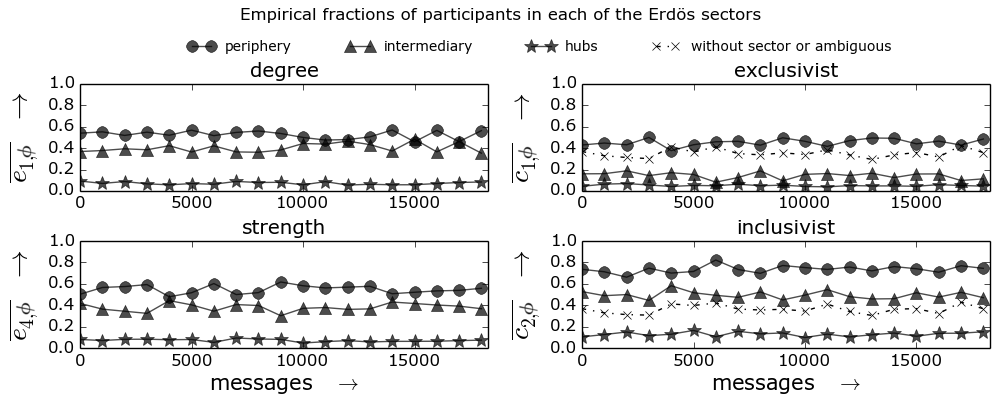
\includegraphics[width=\textwidth]{figs/InText-WLAU-S1000__}
\begin{flushleft}
		Source: Prepared by the authors.\
\end{flushleft}
\label{fig:sectIL}
\end{figure*}


\begin{table}[h]
\caption{Distribution of activity among participants.
The first column shows the percentage of messages sent by the most active participant. The column for the first quartile ($Q_1$) gives the minimum percentage of participants responsible for at least 25\% of total messages with the actual percentage in parentheses. Similarly, the column for the first three quartiles $Q_3$ gives the minimum percentage of participants responsible for 75\% of total messages.
The last decile $D_{-1}$ column shows the maximum percentage of participants responsible for 10\% of messages.}
\begin{center}
\begin{tabular}{ | l ||  c | c | c | c | }
\hline
list & hub & $ Q_1 $ & $ Q_3 $ & $D_{-1}$ \\ \hline
LAU & 2.78  & 1.19 (26.35\%)  & 13.12 (75.17\%)  & 67.32 (-10.02\%) \\
LAD & 4.00  & 1.03 (26.64\%)  & 11.91 (75.18\%)  & 71.14 (-10.03\%) \\
MET & 11.14  & 1.02 (34.07\%)  & 8.54 (75.64\%)  & 80.49 (-10.02\%) \\
CPP & 14.41  & 0.29 (33.24\%)  & 4.18 (75.46\%)  & 83.65 (-10.04\%) \\\hline

\end{tabular}
\end{center}
\begin{flushleft}
		Source: Prepared by the authors.\
\end{flushleft}
\label{autores}
\end{table}


\subsection{Stability of principal components}\label{prevalence}
%The topology was analyzed using standard, well-established metrics of centrality and clustering.
%We also introduced symmetry metrics given the evidence of their importance in social contexts~\cite{newmanEvolving}.
%The contribution of each metric to the variance is very similar for all the networks and along time.

The principal components of the participants are very stable in the topological space,
i.e. in the space of network metrics.
Table~\ref{tab:pcainin} exemplifies the formation of principal components by providing the averages over non-overlapped activity snapshots of a network. The most important result of this application of PCA, the stability of principal components, is underpinned by the very small dispersion of the contribution of each metric to each principal component.
%The contribution of each metric to the
%principal components presents
%very small standard deviation.

\begin{table}[!h]
\caption{Loadings for the 14 metrics into the principal components for the MET list, $1000$ messages in 20 disjoint positions. The clustering coefficient (cc) appears as the first metric in the table, followed by 7 centrality metrics and 6 symmetry-related metrics. Note that the centrality measurements, including degrees, strength and betweenness centrality, are the most important contributors for the first principal component, while the second component is dominated by symmetry metrics. The clustering coefficient is only relevant for the third principal component. The three components have in average more than 85\% of the variance.
The low standard deviation $\sigma$ implies that the principal components are considerably stable.}
\footnotesize
\begin{center}
\begin{tabular}{| l || c | c | c | c | c | c |}\cline{2-7}
\multicolumn{1}{c|}{} & \multicolumn{2}{c|}{PC1}          & \multicolumn{2}{c|}{PC2} & \multicolumn{2}{c|}{PC3}  \\\cline{2-7}\multicolumn{1}{c|}{} & $\mu$            & $\sigma$ & $\mu$         & $\sigma$ & $\mu$ & $\sigma$  \\\hline
$cc$ &                     0.89  & 0.59  & 1.93  & 1.33  & {\bf 21.22}  & 2.97 \\\hline
$s$ &              {\bf 11.71}  & 0.57  & 2.97  & 0.82  & 2.45  & 0.72 \\
$s^{in}$ &         {\bf 11.68}  & 0.58  & 2.37  & 0.91  & 3.08  & 0.78 \\
$s^{out}$ &        {\bf 11.49}  & 0.61  & 3.63  & 0.79  & 1.61  & 0.88 \\
$k$ &              {\bf 11.93}  & 0.54  & 2.58  & 0.70  & 0.52  & 0.44 \\
$k^{in}$ &         {\bf 11.93}  & 0.52  & 1.19  & 0.88  & 1.41  & 0.71 \\
$k^{out}$ &        {\bf 11.57}  & 0.61  & 4.34  & 0.70  & 0.98  & 0.66 \\
$bt$ &             {\bf 11.37}  & 0.55  & 2.44  & 0.84  & 1.37  & 0.77 \\\hline
$asy$ &                    3.14  & 0.98  & {\bf 18.52}  & 1.97  & 2.46  & 1.69 \\
$\mu^{asy}$              & 3.32  & 0.99  & {\bf 18.23}  & 2.01  & 2.80  & 1.82 \\
$\sigma^{asy}$           & 4.91  & 0.59  & 2.44  & 1.47  & {\bf 26.84}  & 3.06 \\
$dis$                    & 2.94  & 0.88  & {\bf 18.50}  & 1.92  & 3.06  & 1.98 \\
$\mu^{dis}$              & 2.55  & 0.89  & {\bf 18.12}  & 1.85  & 1.57  & 1.32 \\
	$\sigma^{dis}$           & 0.57  & 0.33  & 2.74  & 1.63  & {\bf 30.61}  & 2.66 \\\hline\hline
$\lambda$                & 49.56 & 1.16  & 27.14  & 0.54  & 13.25  & 0.95 \\
\hline\end{tabular}
\end{center}

\label{tab:pcainin}
\begin{flushleft}
		Source: Prepared by the authors.\
\end{flushleft}
\end{table}

The first principal component is an average of centrality metrics:
degrees, strengths and betweenness centrality.
On one hand, the similar relevance of all centrality metrics is not surprising since they are highly correlated,
e.g. degree and strength have Spearman correlation coefficient $\in [0.95,1]$ 
and Pearson coefficient $\in [0.85,1)$ for window sizes greater than a thousand messages.
On the other hand, each of these metrics is related to a different participation characteristic,
and their equal relevance for variability,
as measured by the principal component, is noticeable.
Also, this suggests that these centrality metrics 
are equally adequate for characterizing the networks
and the participants.

\begin{figure} 
\centering
%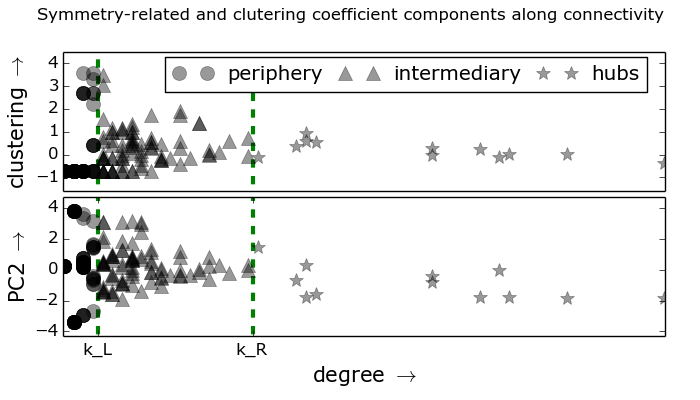
\includegraphics[width=.6\textwidth,height=10cm]{figs/im13PCAPLOT__}
\caption{The first plot highlights the well-known pattern of degree versus clustering coefficient, characterized by the higher clustering coefficient of lower degree vertices.
    The second plot shows the greater dispersion of the symmetry-related ordinates dominant in the second principal component (PC2).
This larger dispersion suggests that symmetry-related metrics are more powerful,
for characterizing interaction networks than the clustering coefficient,
especially for hubs and intermediary vertices.
This figure reflects a snapshot of the LAU list with 1000 contiguous messages.}
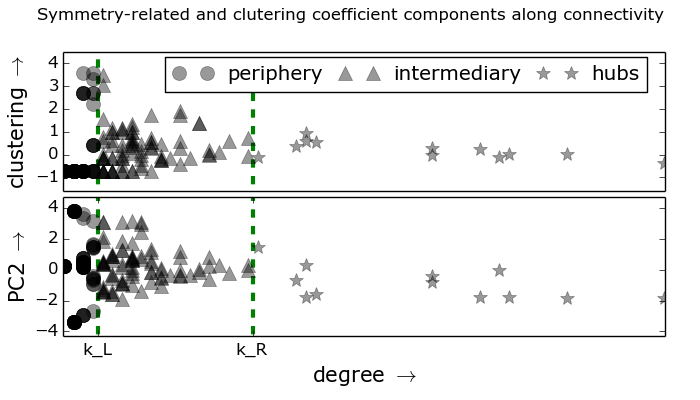
\includegraphics[width=.45\textwidth]{figs/im13PCAPLOT__}

%		Similar structures were observed in all window sizes $ws\;\in\;[500,10000]$, in networks derived from email lists,
%		and in networks from Facebook, Twitter and Participabr,
%		which suggests a common relationship between the metrics of degrees, strengths and betweenness centrality,
%		the symmetry-related metrics and clustering coefficient.}
\label{fig:sym}
\begin{flushleft}
		Source: Prepared by the authors.\
\end{flushleft}
\end{figure}

According to Table~\ref{tab:pcainin} and Figure~\ref{fig:sym},
dispersion is larger in symmetry-related metrics than in clustering coefficient.
% As expected from basic complex network theory, peripheral vertices have low values of centrality metrics and larger dispersion with regard to the clustering coefficient.
% %The scatter plot in the third system of Figure~\ref{fig:sym},
% %where all metrics are considered and there is a greater dispersion
% %with respect to the ordinates,
% This reflects in the relevance of the symmetry-related metrics.
We conclude that the symmetry metrics are more powerful, in terms of dispersion in the topological metrics space, in characterizing interaction networks and their participants, than the clustering coefficient, especially for hubs and intermediary vertices (peripheral vertices have larger dispersion with regard to the clustering coefficient).
Interestingly, the clustering coefficient is always combined
with the standard deviation of the asymmetry and disequilibrium
of edges $\sigma^{asy}$ and $\sigma^{dis}$ in the third principal component.

%These results are also reported for 12 networks from Facebook, Twitter and Participabr
%in Section~\ref{si:ext} of the Supporting Information document.
Similar results are presented in Sections~\ref{si:pcat} and~\ref{si:ext}
of the Appendix for other email lists and interaction networks. A larger variability was found for the latter networks,
which motivated the use of interaction networks derived from email lists for benchmarking.

%the overall behavior was maintained in that centrality measurements 
%were found prevalent in the first principal component,
%followed by symmetry-related metrics on the second principal
%component and then clustering coefficient on the third principal component.
%Similar results are presented in Sections~\ref{si:pcat} and~\ref{si:ext}
%of the Supporting Information document for other email lists and other interaction networks,
%with the consideration of strategic combinations of metrics.

\subsection{Types from Erd\"os sectors}\label{sec:pty}


Assigning a type to a participant raises important issues about the scientific cannon for human types and the potential for stigmatization and prejudice. The Erd\"os sector to which a participant belongs can be regarded as implying a social type for this participant.
In this case, the type of a participant changes both along time and as different networks are considered, despite the stability of the network. Therefore, the potential for prejudice of such participant typology is attenuated~\cite{adorno}. In other words, an individual is a hub in a number of networks and peripheral in other networks, and even within the same network he/she most probably changes type along time~\cite{animacoes}.

The importance of this issue can be grasped by the consideration of static types derived from quantitative criteria. For example, in email lists with a small number of participants, the number of threads has a negative correlation with the number of participants.
When the number of participants exceeds a threshold, the number of threads has a positive correlation with the number of participants.
This finding is illustrated in Figure~\ref{fig:nmgamma3d}
and can also be observed in Table~\ref{tab:genLists}.
The assignment of types to individuals, in this latter case,
has more potential for prejudice because
the derived participant type is static and
one fails to acknowledge that
human individuals are not immutable entities.

Further observations regarding the Erd\"os sectors
and the implicit participant types were made, which are consistent with the literature~\cite{barabasiEvo}: 1) hubs and intermediary participants usually have intermittent activity, and stable activity was found only in smaller communities. For instance, the MET list had stable hubs while LAU, LAD and CPP exhibited intermittent hubs.
2) Network structure seems to be most influenced by the
activity of intermediary participants as they have less extreme
roles than hubs and peripheral participants and
can therefore connect to the sectors and other participants 
in a more selective and explicit manner.




%Moreover, such typology of participants bridges exact and human sciences and may 
%be enriched with concepts from other typologies,
%such as Meyer-Briggs, Pavlov or the authoritarian types of the F-Scale~\cite{adorno}.

%We analyzed the temporal evolution of the networks
%using visualization
%tools developed for this research~\cite{rcText,versinus}
%and inspected raw data.

%dictated (or revealed) by the
%(e.g. stable or intermittent patterns of activity and preferential communication
%with hubs or periphery)

%of both hubs and peripheral vertices
%have the trivial facets of interacting 
%
%
%
%\begin{itemize}
%	\item Typically, the activity of hubs is trivial: they interact as much as possible, in every occasion with everyone.
%The activity of peripheral vertices also follows a simple pattern: they interact very rarely, in very few occasions.
%Therefore, intermediary vertices seem responsible for the network structure.
%Intermediary vertices may exhibit preferential communication to peripheral, intermediary, or hub vertices; can be marked by stable communication partners; can involve stable or intermittent patterns of activity, to point just a few examples of this greater variety of roles.
%%	\item Some of the most active participants receive many responses with relative few messages sent, and rarely are top hubs.
%%These seem as authorities and contrast with participants that respond much more than receive responses.
%%	\item The most obvious community structure, as observed by a high clustering coefficient, i.e. members know each other often, is found mostly in peripheral and intermediary sectors.
%\end{itemize}

%Within networks as the whole objects of analysis,
%we were able to observe a peculiar correlation pattern 
%between the number of threads and the number of participants.
\begin{figure}
\centering
\caption{A scatter plot of number of messages $M$ versus number of participants $N$ versus number of threads $\Gamma$ for 140 email lists.
Highest $\Gamma$ is associated with low $N$.
The correlation between $N$ and $\Gamma$ is negative for low values of $N$ but positive otherwise.
This negative correlation between $N$ and $\Gamma$ can also be observed in Table~\ref{tab:genLists}.
Accordingly, for $M=20000$ messages, this inflection
of correlation was found around $N=1500$, while CPP, LAU, LAD, MET lists 
present smaller networks.}
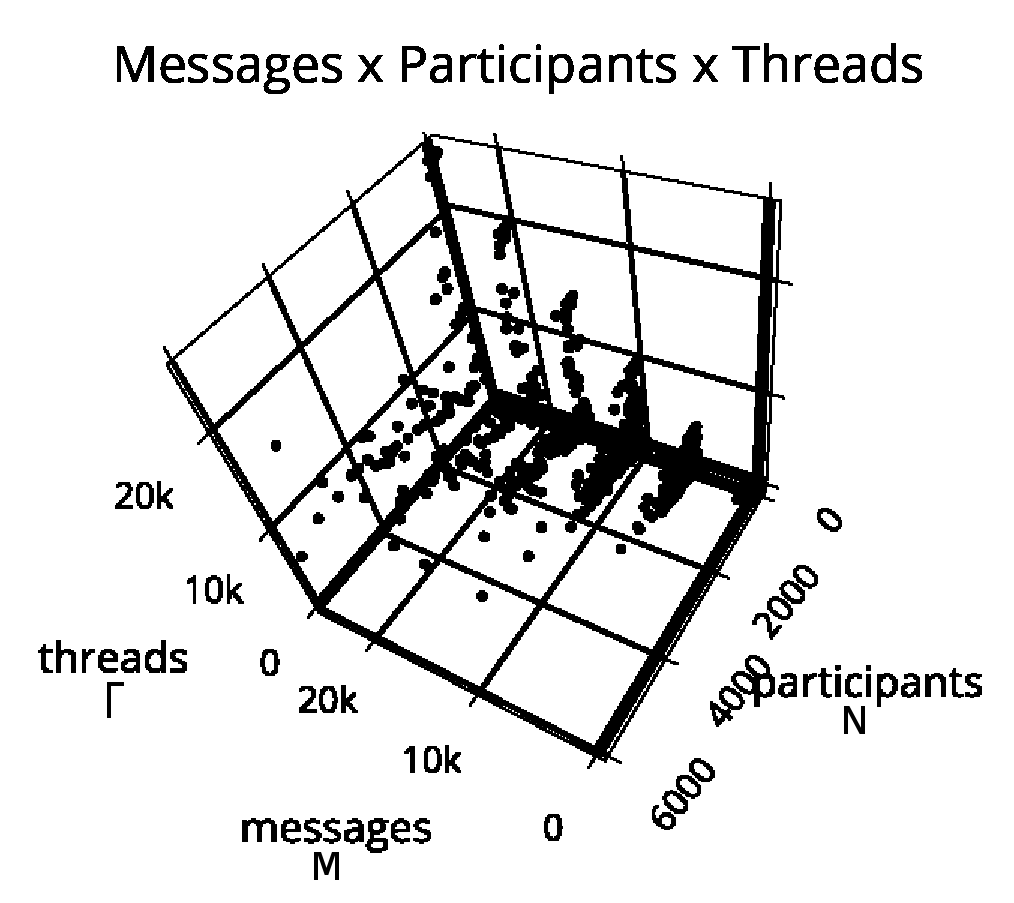
\includegraphics[trim={0 0 0 1cm},clip,width=.7\columnwidth]{figs/mpgamma2_}
\begin{flushleft}
		Source: Prepared by the authors.\
\end{flushleft}
\label{fig:nmgamma3d}
\end{figure}


%\section{Discussion}
% given the results, and before reaching the conclusions
% what to say?
% --> what is the overall knowledge derived from the results
% --> what are the limitations of this knowledge and of individual results
% --> how should this results carry on is on the next sections.
%\subsection{Consecutive scientific research}
% --> research
% textual diferences
% audiovisualization of data
% typologies, sociological critical theory, social psychology

%\subsection{Technological applications}
% --> technological 
% resources categorization and recommendation
% document creation
% ontologies for the semantic web

%\subsection{Experimental and theoretical aspects of the research}
% --> methods
% Exploratory?
% Hypothesis testing?
% --> contributions
% verifiable
% knowledge
% contextualization in the academic knowledge

\subsection{Implications of the main findings}\label{sec:impl}
The findings reported in this thesis arose from an exploratory procedure to visually inspect the networks and to analyze considerable amounts of interaction networks data.
% deriving from email lists and also from other networks.
While this procedure has certainly an ad hoc nature, the statistics in the data are sufficiently robust for important features from these interaction networks to be extracted.
Temporal stability, in the sense that interaction networks could be considered as stationary time series, is the most important feature. Also relevant is the significant stability found on the principal components, on the fraction of participants in each Erd\"os Sector and on the activity along different timescales. In fact, these findings confirm our initial hypothesis - based on the literature~\cite{newmanBook} - that interaction networks should exhibit some stability traces. The potential generality of these findings is suggested by the analysis of networks derived from diverse systems, with interaction networks from public email lists serving as proper benchmarks. Indeed, with such benchmarks one can compare any social network system. Furthermore, this analysis enables us to establish an outline of human interaction networks. It takes the hub, intermediary and periphery sectors out of the scientific folklore and into classes drawn from quantitative criteria. It enables the conception of non-static human types derived from natural properties.

 
We envisage that the knowledge generated in the analysis may be exploited in applications where the type of each participant and the relative proportion of participants in each sector can be useful metadata. Just by way of illustration, this could be applied in semantic web initiatives, given that the Erd\"os sectorialization is static in a given snapshot. These results are also useful for classifying resources, e.g. in social media, and for resources recommendation to users~\cite{opa}. 
Finally, the knowledge acquired with a quantitative treatment of the whole data may help guide the creation through collective processes of documents to assist in participatory democracy.

 
Perhaps the most outreaching implications are related to sociological consequences. The results expose a classification of human individuals which is directly related to the concentration of wealth and based on natural laws. The derived human typology changes over different systems and over time in the same system, which implies a negation of the absolute concentration of wealth. Such concentration exists but changes across different wealth criteria and with time. Also, the hubs stand out as dedicated, sometimes enslaved,
components of the social system. The peripheral participants have very limited interaction with the network. This suggests that intermediary participants tend to dictate structure, legitimate the hubs and stand out as authorities.

 
With regard to the limitations of our study, one should emphasize that not all types of human interaction networks were analyzed. Therefore, the plausible generalization of properties has to be treated with caution, as a natural tendency of such systems and not as a rule. Also, the stable properties in the networks were not explored to the limit, which leaves many open questions. For example, what are the maximum and minimum sizes of the networks for which they hold? What is the outcome of PCA when more metrics are considered? What is the granularity in which the activity along the timescales is preserved? Do the findings reported also apply to other systems, beyond human networks?
 
 % TTM find
\section{Text-related results and discussion}\label{sec:tresults}
% Aqui será necessária uma Introdução a este novo tipo de resultado.

The most important result of including textual metrics in our analysis is the
statistical evidence of extreme differentiation of each Erd\"os sector with respect to the texts produced.
This conclusion can be reached by observing the differences in the measurements of textual features in
each sector, but is reached with greater theoretical background from the adaptation of the
Kolmogorov-Smirnov test we presented in Section~\ref{sec:ks}.
% derived from the kolmogorov-smirnov test adaptation
Other relevant results are:
\begin{itemize}
	\item the achievement of references for the amount of nouns, adverbs, sizes of words, depth of Wordnet synsets and other linguistic traces, used in social networks.
		We did not find in literature any indication for such values and understood useful to acknowledge e.g. that about 15\% of the characters are spaces and more than 50\% of tokens are nouns.
		These values are available in~\cite{textTables} and not in the body of the text,
		since we focus in this thesis in the evidence that the texts from distinct sectors differ.
	\item Indicatives of what is different in the texts produced by each of the Erd\"os sectors.
		For example: hubs were found to use more contractions,
		more common words, and less punctuation if compared to the rest of the network,
		especially the peripheral sector.
		In general, the rise or fall of a text-related metric is not relevant or is monotonic along connectivity,
		but some of them reaches extreme values in the intermediary sector.
		% Comparative insights by means of statistics from email lists, the King James Bible and Shakespeare, which are often regarded as pillars of the English language. TTM
\end{itemize}

The next sections summarize results of immediate interest
and further insights can be obtained by skimming through
the tables and figures of~\cite{stab,textTables} and the Conclusions chapter.
We illustrate with just one table of each kind,
and from networks obtained with 2000 messages.
In~\cite{textTables} we display tables for various networks.
In the same document, we relate the email lists to each numerical
TAG in the tables of the following sections.
The scale of 1000 and 2000 messages was chosen for deriving results,
as the networks in this scale are found with stable topological structure,
as exposed in Section~\ref{subsec:pih}.
The findings with 1000 messages are the same as with 2000 messages,
and there are many tables.
This motivated the exclusion of the tables with measurements in
networks of 1000 messages.

\subsection{General characteristics of activity distribution among sectors}\label{sec:gen}
Before we dig into the findings derived from text-related measures,
let us look once more at the general structure of these networks,
now giving emphasis on the activity of the sectors.
In almost all our observations,
the peripheral sector is responsible for starting most of the discussion threads,
i.e. messages to the list which are not replies.
This is surprising since the peripheral sector is responsible for fewer messages.
This suggests a complementarity between peripheral diversity and hub specialization
which, on its turn, deepens the understanding of the interaction network as a meaningful system. 
These assertions are condensed in Table~\ref{geralListas}.
Less often, the intermediary sector is responsible for the greatest number of messages
and of threads.
Also meaningful is that the hubs sector is responsible for most of the messages,
which is not completely obvious: hub participants are far more active but way less numbered.
Interestingly, in such a setting where every characteristic differs with respect to
distinct sectors, there was no evidence of difference on the size of the threads started by each sector.
\begin{table}[h!]
\begin{center}
\caption{Distribution of participants, messages and threads among each Erd\"os sector ({\bf p.} for periphery, {\bf i.} for intermediary, 
    {\bf h.} for hubs) in a total timespan of 0.72 years (from 2003-11-30T20:21:32 to 2004-08-19T18:11:24). $N$ is the number of participants, $M$ is the number of messages, $\Gamma$ is the number of threads, and $\gamma$ is the number of messages in a thread.
    The \% denotes the usual `per cent' with respecto to the total quantity ($100\%$ for {\bf g.})
    while $\mu$ and $\sigma$ denote mean and standard deviation. TAG of list in the Appendix~\ref{ap:texttop}: 10}\label{geralListas}    
\begin{tabular}{| l || c | c | c | c |}\hline
 & {\bf g.} & {\bf p.} & {\bf i.} & {\bf h.} \\\hline\hline
$N$ & 131  & 80  & 46  & 5 \\
$N_{\%}$ & 100.00  & 61.07  & 35.11  & 3.82 \\\hline
$M$ & 1000.00  & 136.00  & 361.00  & 503.00 \\
$M_{\%}$ & 100.00  & 13.60  & 36.10  & 50.30 \\\hline
$\Gamma$ & 292.00  & 76.00  & 147.00  & 69.00 \\
$\Gamma_{\%}$ & 100.00  & 26.03  & 50.34  & 23.63 \\\hline
$\frac{\Gamma}{M}\%$ & 29.20  & 55.88  & 40.72  & 13.72 \\
$\mu(\gamma)$ & 2.74  & 2.76  & 2.81  & 2.58 \\
$\sigma(\gamma)$ & 0.44  & 0.43  & 0.39  & 0.49 \\\hline
\end{tabular}
\end{center}
\begin{flushleft}
		Source: Prepared by the authors.\
\end{flushleft}
\end{table}


%Also, comparing lists with a fixed number of messages,
%the number of threads created seem to increase as the number of participants decrease.

\subsection{Evidence that the texts from Erd\"os sectors differ}\label{subsec:di}
Results from our adaptation of the Kolmogorov-Smirnov test (see Section~\ref{sec:ks})
present substantial evidence
that the texts produced by each sector are different.
Tables~\ref{tab:kolTok}-\ref{tab:kolPctInter}
illustrate three results:
\begin{itemize}
    \item There is statistical evidence that the textual production of the Erd\"os sectors are different.
	    This can be noticed from the high values of $c'$ on these tables,
	    beyond reference values used for the acceptance of the 
	    null hypothesis.
		Also, we regarded as non-negligible 
		the values often above 0.1 for the Kolmogorov-Smirnov statistic (the maximum difference between the cumulative distributions),
		which we recognized as relevant for assuming differences in the underlying distributions in our study (see Section~\ref{sec:ks}).
    \item Intermediary sectors sometimes exhibit greater differences 
from periphery and hubs than these extreme sectors between themselves 
(Tables~\ref{tab:kolTok} and~\ref{tab:kolSub}).
This differentiation of the three sectors is an
indicative that the Erd\"os Sectioning
described in Section~\ref{sectioning} reveals meaningful
sectors of the networks.
    \item Evidence of differences between sectors on the same network 
	    (Tables~\ref{tab:kolTok}-\ref{tab:kolPct}) is often greater than differences between the same sector from distinct lists (Tables~\ref{tab:kolSubInter}-\ref{tab:kolPctInter}).
\end{itemize}

\begin{table}[h!]
\begin{center}
\caption{KS distances on size of tokens. TAG: 6}
	\label{tab:kolTok}
\begin{tabular}{| l || c | c | c | c |}\hline
 & {\bf g.} & {\bf p.} & {\bf i.} & {\bf h.} \\\hline\hline
{\bf g.} & 0.000 & 4.327 & 17.168 & 7.851 \\
{\bf } & 0.000 & 0.014 & 0.115 & 0.044 \\\hline
{\bf p.} & 4.327 & 0.000 & 18.907 & 7.833 \\
{\bf } & 0.014 & 0.000 & 0.129 & 0.045 \\\hline
{\bf i.} & 17.168 & 18.907 & 0.000 & 15.540 \\
{\bf } & 0.115 & 0.129 & 0.000 & 0.129 \\\hline
{\bf h.} & 7.851 & 7.833 & 15.540 & 0.000 \\
{\bf } & 0.044 & 0.045 & 0.129 & 0.000 \\\hline
\end{tabular}
\begin{flushleft}
		Source: By the author.\
\end{flushleft}
\end{center}
\end{table}

\begin{table}[h!]
\begin{center}
\caption{KS distances on size of known words. TAG: 1}
\begin{tabular}{| l || c | c | c | c |}\hline
 & {\bf g.} & {\bf p.} & {\bf i.} & {\bf h.} \\\hline\hline
{\bf g.} & 0.000 & 5.904 & 5.264 & 5.549 \\
{\bf } & 0.000 & 0.043 & 0.040 & 0.150 \\\hline
{\bf p.} & 5.904 & 0.000 & 9.547 & 7.073 \\
{\bf } & 0.043 & 0.000 & 0.083 & 0.193 \\\hline
{\bf i.} & 5.264 & 9.547 & 0.000 & 4.058 \\
{\bf } & 0.040 & 0.083 & 0.000 & 0.111 \\\hline
{\bf h.} & 5.549 & 7.073 & 4.058 & 0.000 \\
{\bf } & 0.150 & 0.193 & 0.111 & 0.000 \\\hline
\end{tabular}
\begin{flushleft}
		Source: Prepared by the authors.\
\end{flushleft}
\end{center}
\end{table} 

\begin{table}[h!]
\begin{center}
\caption{KS distances on size of sentences. TAG: 2}
\begin{tabular}{| l || c | c | c | c |}\hline
 & {\bf g.} & {\bf p.} & {\bf i.} & {\bf h.} \\\hline\hline
{\bf g.} & 0.000 & 0.733 & 2.077 & 2.834 \\
{\bf } & 0.000 & 0.020 & 0.038 & 0.059 \\\hline
{\bf p.} & 0.733 & 0.000 & 1.642 & 2.589 \\
{\bf } & 0.020 & 0.000 & 0.048 & 0.080 \\\hline
{\bf i.} & 2.077 & 1.642 & 0.000 & 4.139 \\
{\bf } & 0.038 & 0.048 & 0.000 & 0.097 \\\hline
{\bf h.} & 2.834 & 2.589 & 4.139 & 0.000 \\
{\bf } & 0.059 & 0.080 & 0.097 & 0.000 \\\hline
\end{tabular}
\begin{flushleft}
		Source: Prepared by the author.\
\end{flushleft}
\end{center}
\end{table}


\begin{table}[h!]
\begin{center}
\caption{KS distances on use of adjectives on sentences. TAG: 3}
\begin{tabular}{| l || c | c | c | c |}\hline
 & {\bf g.} & {\bf p.} & {\bf i.} & {\bf h.} \\\hline\hline
{\bf g.} & 0.000 & 0.461 & 0.564 & 0.617 \\
{\bf } & 0.000 & 0.011 & 0.010 & 0.010 \\\hline
{\bf p.} & 0.461 & 0.000 & 0.385 & 0.800 \\
{\bf } & 0.011 & 0.000 & 0.011 & 0.021 \\\hline
{\bf i.} & 0.564 & 0.385 & 0.000 & 0.986 \\
{\bf } & 0.010 & 0.011 & 0.000 & 0.020 \\\hline
{\bf h.} & 0.617 & 0.800 & 0.986 & 0.000 \\
{\bf } & 0.010 & 0.021 & 0.020 & 0.000 \\\hline
\end{tabular}
\begin{flushleft}
		Source: Prepared by the author.\
\end{flushleft}
\end{center}
\end{table}

\begin{table}[h!]
\begin{center}
\caption{KS distances on use of substantives on sentences. TAG: 1}
\begin{tabular}{| l || c | c | c | c |}\hline
 & {\bf g.} & {\bf p.} & {\bf i.} & {\bf h.} \\\hline\hline
{\bf g.} & 0.000 & 0.642 & 1.791 & 6.936 \\
{\bf } & 0.000 & 0.023 & 0.067 & 0.537 \\\hline
{\bf p.} & 0.642 & 0.000 & 1.007 & 6.970 \\
{\bf } & 0.023 & 0.000 & 0.044 & 0.560 \\\hline
{\bf i.} & 1.791 & 1.007 & 0.000 & 7.510 \\
{\bf } & 0.067 & 0.044 & 0.000 & 0.607 \\\hline
{\bf h.} & 6.936 & 6.970 & 7.510 & 0.000 \\
{\bf } & 0.537 & 0.560 & 0.607 & 0.000 \\\hline
\end{tabular}
\end{center}
\begin{flushleft}
		Source: Prepared by the authors.\
\end{flushleft}
\end{table}

\begin{table}[h!]
\begin{center}
\caption{KS distances on use of punctuations on sentences. TAG: 8}
	\label{tab:kolPct}
\begin{tabular}{| l || c | c | c | c |}\hline
 & {\bf g.} & {\bf p.} & {\bf i.} & {\bf h.} \\\hline\hline
{\bf g.} & 0.000 & 1.380 & 3.583 & 2.894 \\
{\bf } & 0.000 & 0.039 & 0.069 & 0.046 \\\hline
{\bf p.} & 1.380 & 0.000 & 1.718 & 2.871 \\
{\bf } & 0.039 & 0.000 & 0.054 & 0.085 \\\hline
{\bf i.} & 3.583 & 1.718 & 0.000 & 5.398 \\
{\bf } & 0.069 & 0.054 & 0.000 & 0.114 \\\hline
{\bf h.} & 2.894 & 2.871 & 5.398 & 0.000 \\
{\bf } & 0.046 & 0.085 & 0.114 & 0.000 \\\hline
\end{tabular}
\begin{flushleft}
		Source: Prepared by the author.\
\end{flushleft}
\end{center}
\end{table}

\begin{table}
  \centering
  \caption{$c'$ values for substantives. Comparison of the same sector between lists, each author is an observation. See subsection~\ref{subsec:di} for discussion and directions.}
    \small
\setlength{\tabcolsep}{.06667em}
  \begin{tabular}{|l|| c|c|c|c|c|c|}\hline
& CPP-LAD & CPP-LAU & CPP-ELE & LAD-LAU & LAD-ELE & LAU-ELE \\\hline
P & 1.35 & 4.05 & 5.80 & 3.00 & 5.41 & 4.94 \\\hline
I & 1.27 & 0.78 & 4.01 & 0.84 & 3.84 & 3.94 \\\hline
H & 0.98 & 1.94 & 3.17 & 1.32 & 3.82 & 4.47 \\\hline
  \end{tabular}
\begin{flushleft}
		Source: Prepared by the authors.\
\end{flushleft}
  \label{tab:kolSubInter}
\end{table}

\begin{table}
  \centering
  \caption{$c'$ values for adjectives. Comparison of the same sector between lists, each author is an observation. See subsection~\ref{subsec:di} for discussion and directions.}
    \small
\setlength{\tabcolsep}{.06667em}
  \begin{tabular}{|l|| c|c|c|c|c|c|}\hline
 & CPP-LAD & CPP-LAU & CPP-ELE & LAD-LAU & LAD-ELE & LAU-ELE \\\hline
P & 0.44 & 0.34 & 2.57 & 0.20 & 2.32 & 2.37 \\\hline
I & 0.74 & 0.99 & 3.72 & 0.32 & 3.37 & 3.10 \\\hline
H & 0.26 & 0.32 & 3.72 & 0.29 & 4.36 & 4.24 \\\hline
  \end{tabular}
\begin{flushleft}
		Source: Prepared by the authors.\
\end{flushleft}
  \label{tab:kolAdjInter}
\end{table}

\begin{table}
  \centering
  \caption{$c'$ values for stopwords. Comparison of the same sector between lists, each author is an observation. See subsection~\ref{subsec:di} for discussion and directions.}
    \small
\setlength{\tabcolsep}{.06667em}
  \begin{tabular}{|l|| c|c|c|c|c|c|}\hline
 & CPP-LAD & CPP-LAU & CPP-ELE & LAD-LAU & LAD-ELE & LAU-ELE \\\hline
P & 3.31 & 3.26 & 6.68 & 0.57 & 5.36 & 5.41 \\\hline
I & 1.45 & 1.08 & 5.16 & 0.91 & 5.00 & 4.92 \\\hline
H & 0.98 & 0.68 & 4.35 & 1.05 & 4.73 & 5.01 \\\hline
  \end{tabular}
\begin{flushleft}
		Source: Prepared by the authors.\
\end{flushleft}
  \label{tab:kolSwInter}
\end{table}

\begin{table}
  \centering
  \caption{$c'$ values for punctuations/char. Comparison of the same sector between lists, each author is an observation. See subsection~\ref{subsec:di} for discussion and directions.}
    \small
\setlength{\tabcolsep}{.06667em}
  \begin{tabular}{|l|| c|c|c|c|c|c|}\hline
 & CPP-LAD & CPP-LAU & CPP-ELE & LAD-LAU & LAD-ELE & LAU-ELE \\\hline
P & 5.74 & 4.88 & 8.28 & 2.23 & 5.37 & 6.60 \\\hline
I & 3.23 & 2.49 & 4.16 & 0.96 & 3.40 & 3.51 \\\hline
H & 2.49 & 1.87 & 4.02 & 1.36 & 3.05 & 3.71 \\\hline
  \end{tabular}
\begin{flushleft}
		Source: Prepared by the authors.\
\end{flushleft}
  \label{tab:kolPctInter}
\end{table}
 


\FloatBarrier
\subsection{What and how the texts from the sectors differs}
In the next sections we will look through text-related measures
and summarize the findings about what might be different in
the textual features of the sectors.
One should keep in mind that our core result is the evidence that
the texts from distinct sectors differ.
The following discussion of what differs and how it differs
is interesting but is both derived from less strong statistical evidence
and less crucial for our current stage of researching these structures.
Nonetheless, for the sake of clarity, we state the main findings:
\begin{itemize}
	\item Peripherals use more nouns while hubs use more verbs and adverbs.
		The fraction of adjectives did not change systematically with respect to connectivity,
		but given that the nouns are more numerous in the periphery, there are more adjectives per noun in the hubs sector texts.
	\item The size of tokens and words were found greater in the more connected sectors,
		which might be related to the use of a more specialized vocabulary.
		Sentences and messages were found smaller in the more connected sectors.
	\item The differences found with respect to Wordnet synsets were found less well behaved.
		Often, the sectors exhibit noticeable differences but greater and smaller incidences are found in all sectors (but in different networks).
		Some incidences are more systematic and this analysis assisted by Wordnet is semantic, reasons that motivated our inclusion of these results by means not of example tables but by explicit counts of greater incidence in each sector throughout the networks.
\end{itemize}


% We can summarize these results stating that the difference
% found between texts from distinct Erd\"os sectors
% is further evidenced.
% We can summarize these results stating that the difference
% found between the texts produced by the Erd\"os sectors
% are greater than the difference found between texts from different
% networks or from the same sector of different networks.

\subsection{Characters}\label{sec:cha}
Most often, peripheral and intermediary sectors use more digits and upper case letters.
Hubs use more letters and vowels among letters.
The use of white spaces, for example, does not seem to have any relation to connectivity. 
These results are illustrated in Table~\ref{tab:cha}.
\begin{table}[h!]
\begin{center}
\begin{tabular}{| l || c | c | c | c |}\hline
 & {\bf g.} & {\bf p.} & {\bf i.} & {\bf h.} \\\hline\hline
$chars$ & 1485813  & 552986  & 554328  & 378499 \\
$chars_{\%}$ & 100.00  & 37.22  & 37.31  & 25.47 \\\hline
$\frac{spaces}{chars}$ & 12.94  & 12.79  & 12.82  & 13.35 \\
$\frac{punct}{chars-spaces}$ & 9.54  & 10.53  & 10.15  & 7.20 \\
$\frac{digits}{chars-spaces}$ & 4.49  & 7.13  & 3.87  & 1.54 \\\hline
$\frac{letters}{chars-spaces}$ & 83.95  & 80.09  & 83.95  & 89.65 \\
$\frac{vowels}{letters}$ & 36.94  & 36.10  & 36.98  & 38.00 \\
$\frac{uppercase}{letters}$ & 4.49  & 4.60  & 4.68  & 4.07 \\\hline
\end{tabular}
\caption{Characters in each Erd\"os sector ({{\bf p.}} for periphery, {{\bf i.}} for intermediary, 
	{{\bf h.}} for hubs). TAG: 6}\label{tab:cha}
\end{center}
\end{table}

\FloatBarrier
% The total number of characters in ELE list,
% in the 20 thousand messages,
% is more than three times what other lists exhibited.
% This suggests peculiarities related to communication conventions and style (see Appendix~\ref{sec:materials}) and were found not related to topological features.

\subsection{Tokens and words}\label{subsec:tw}
%\begin{table}[h!]
\begin{center}
\begin{tabular}{| l || c | c | c | c |}\hline
 & {\bf g.} & {\bf p.} & {\bf i.} & {\bf h.} \\\hline\hline
$tokens$ & 17964  & 1539  & 6064  & 10361 \\
$tokens_{\%}$ & 100.00  & 8.57  & 33.76  & 57.68 \\
$tokens \neq$ & 15.21  & 32.16  & 25.89  & 18.02 \\\hline
$\frac{knownw}{tokens}$ & 36.48  & 35.74  & 38.03  & 35.69 \\
$\frac{knownw \neq}{knownw}$ & 8.62  & 24.73  & 15.31  & 10.84 \\\hline
$\frac{stopw}{knownw}$ & 11.43  & 10.00  & 11.71  & 11.47 \\
$\frac{punct}{tokens}$ & 23.73  & 22.35  & 22.82  & 24.47 \\
$\frac{contrac}{tokens}$ & 0.01  & 0.00  & 0.00  & 0.02 \\\hline
\end{tabular}
\caption{tokens in each Erd\"os sector ({{\bf p.}} for periphery, {{\bf i.}} for intermediary, 
    {{\bf h.}} for hubs).}
\end{center}
\end{table}

%The largest average size of tokens is from the most wordy list (ELE).
%This implies that is has more characters, tokens, and characters per token in comparison to the other lists. 
In most of the networks analyzed, hubs use longer words, which might be related to the use of a specialized vocabulary.
Hubs use more contractions and known words, while peripheral sector exhibit a greater incidence of punctuations among tokens.
Although the token diversity ($\frac{|tokens \neq|}{|tokens|}$) found in peripheral sector is far greater,
this result has the masking artifact that the peripheral sector corpus is smaller, yielding a larger token diversity.
This can be noticed by the token diversity of the whole network, which is lower than in any of the sectors.
The same observation apply to the lexical diversity ($\frac{|kw\neq|}{kw}$).
These results are exemplified in Table~\ref{tab:tokensInline}
where mean and variance were taken with respect to the length in characters of tokens, known words and stopwords.
\begin{table}[h!]
\begin{center}
\begin{tabular}{| l || c | c | c | c |}\hline
 & {\bf g.} & {\bf p.} & {\bf i.} & {\bf h.} \\\hline\hline
$tokens$ & 286232  & 146472  & 134852  & 4908 \\
$tokens_{\%}$ & 100.00  & 51.17  & 47.11  & 1.71 \\
$tokens \neq$ & 3.00  & 4.01  & 3.66  & 24.08 \\\hline
$\frac{knownw}{tokens}$ & 25.76  & 25.11  & 26.21  & 32.84 \\
$\frac{knownw \neq}{knownw}$ & 4.51  & 6.22  & 5.92  & 42.80 \\\hline
$\frac{stopw}{knownw}$ & 42.46  & 38.92  & 43.60  & 98.33 \\
$\frac{punct}{tokens}$ & 33.18  & 34.09  & 32.56  & 23.11 \\
$\frac{contrac}{tokens}$ & 0.16  & 0.10  & 0.18  & 1.67 \\\hline\hline
$\mu(\overline{tokens})$ & 3.19  & 3.10  & 3.26  & 3.65 \\
$\sigma(\overline{tokens})$ & 2.53  & 2.54  & 2.52  & 2.60 \\\hline
$\mu(\overline{knownw})$ & 4.89  & 4.69  & 5.06  & 5.50 \\
$\sigma(\overline{knownw})$ & 2.37  & 2.41  & 2.31  & 2.28 \\\hline
$\mu(\overline{knownw \neq})$ & 6.53  & 6.39  & 6.27  & 6.16 \\
$\sigma(\overline{knownw \neq})$ & 2.53  & 2.50  & 2.46  & 2.42 \\\hline
$\mu(\overline{stopw})$ & 2.83  & 2.83  & 2.83  & 2.81 \\
$\sigma(\overline{stopw})$ & 0.87  & 0.84  & 0.86  & 1.17 \\\hline
\end{tabular}
	\caption{Tokens in each Erd\"os sector ({{\bf p.}} for periphery, {{\bf i.}} for intermediary, {{\bf h.}} for hubs). TAG: 1}\label{tab:tokensInline}
\end{center}
\end{table}

\FloatBarrier
% medir para tamanhos equivalentes de texto TTM

% ELE and CPP both exhibit intermediaries 
% with the more frequent production of punctuation,
% less frequent production of known words, and
% the highest incidence of words with wordnet synsets among known words.
% This suggests some peculiarity in network structure,
% such as authorities in the intermediary sector of such networks,
% using smaller sentences and a more intensive use of jargons,
% as made explicit in the following sections.
% verificar isso e ver o que fazer

% Words with synsets,
% among known English words, are less frequent in hubs sector,
% evidencing the jargon and specialization of hubs.
% verificar, desenvolvar

%\begin{table}[h!]
\begin{center}
\begin{tabular}{| l || c | c | c | c |}\hline
 & {\bf g.} & {\bf p.} & {\bf i.} & {\bf h.} \\\hline\hline
$\mu(\overline{tokens})$ & 3.84  & 3.94  & 3.86  & 3.82 \\
$\sigma(\overline{tokens})$ & 2.99  & 3.10  & 2.96  & 2.99 \\\hline
$\mu(\overline{knownw})$ & 3.28  & 3.27  & 3.32  & 3.26 \\
$\sigma(\overline{knownw})$ & 1.81  & 1.86  & 1.80  & 1.81 \\\hline
$\mu(\overline{knownw \neq})$ & 5.12  & 4.35  & 4.92  & 4.98 \\
$\sigma(\overline{knownw \neq})$ & 2.20  & 2.22  & 2.25  & 2.15 \\\hline
$\mu(\overline{stopw})$ & 1.77  & 1.84  & 1.77  & 1.76 \\
$\sigma(\overline{stopw})$ & 0.74  & 0.76  & 0.73  & 0.75 \\\hline
\end{tabular}
\caption{Token sizes in each Erd\"os sector ({{\bf p.}} for periphery, {{\bf i.}} for intermediary, {{\bf h.}} for hubs).}
\end{center}
\end{table}

\subsection{Sizes of sentences}\label{subsec:ss}
Hubs present the lowest average sentence size,
in characters, tokens or known words.
This result is illustrated in Table~\ref{tab:sizesSents}
and might be considered counterintuitive given that punctuation
is more abundant in the texts of less connected participants.
\begin{table}[h!]
\begin{center}
	\caption{Sentences sizes in each Erd\"os sector ({{\bf p.}} for periphery, {{\bf i.}} for intermediary, {{\bf h.}} for hubs). TAG: 16}\label{tab:sizesSents}
\begin{tabular}{l || c | c | c | c}\hline
 & {\bf g.} & {\bf p.} & {\bf i.} & {\bf h.} \\\hline\hline
$sents$ & 10757  & 1252  & 4529  & 4978 \\
$sents_{\%}$ & 99.98  & 11.64  & 42.09  & 46.27 \\\hline
$\mu_S(chars)$ & 113.88  & 143.37  & 120.21  & 100.65 \\
$\sigma_S(chars)$ & 318.65  & 750.47  & 276.21  & 88.88 \\\hline
$\mu_S(tokens)$ & 24.78  & 28.83  & 26.72  & 21.98 \\
$\sigma_S(tokens)$ & 40.56  & 77.72  & 42.08  & 20.23 \\\hline
$\mu_S(knownw)$ & 7.81  & 8.37  & 8.26  & 7.25 \\
$\sigma_S(knownw)$ & 8.18  & 9.38  & 9.30  & 6.56 \\\hline
$\mu_S(stopw)$ & 7.78  & 7.61  & 7.92  & 7.70 \\
$\sigma_S(stopw)$ & 6.88  & 6.94  & 7.36  & 6.39 \\\hline
$\mu_S(puncts)$ & 4.29  & 5.42  & 5.04  & 3.33 \\
$\sigma_S(puncts)$ & 9.92  & 13.08  & 12.13  & 5.82 \\\hline
\end{tabular}
\begin{flushleft}\footnotesize
		Source: By the author.\
\end{flushleft}
\end{center}
\end{table}

\FloatBarrier

\subsection{Messages}\label{subsec:mm}
Connectivity was found correlated to smaller messages in terms of characters and tokens.
Connectivity was also found correlated to smaller messages in terms of the number of sentences, but
it was less consistent.
This result is exemplified in Table~\ref{tab:sizesMsgs}.
\begin{table}[h!]
\begin{center}
	\caption{Messages sizes in each Erd\"os sector ({{\bf p.}} for periphery, {{\bf i.}} for intermediary, {{\bf h.}} for hubs). TAG: 0}\label{tab:sizesMsgs}
\begin{tabular}{| l || c | c | c | c |}\hline
 & {\bf g.} & {\bf p.} & {\bf i.} & {\bf h.} \\\hline\hline
$msgs$ & 1992  & 286  & 841  & 865 \\
$msgs_{\%}$ & 100.00  & 14.36  & 42.22  & 43.42 \\\hline
$\mu_M(sents)$ & 5.21  & 6.08  & 6.43  & 3.74 \\
$\sigma_M(sents)$ & 6.78  & 4.03  & 9.40  & 3.26 \\\hline
$\mu_M(tokens)$ & 145.82  & 230.45  & 186.07  & 78.71 \\
$\sigma_M(tokens)$ & 260.61  & 291.17  & 326.68  & 127.13 \\\hline
$\mu_M(knownw)$ & 38.83  & 56.29  & 48.87  & 23.29 \\
$\sigma_M(knownw)$ & 50.54  & 58.28  & 58.67  & 31.16 \\\hline
$\mu_M(stopw)$ & 34.29  & 41.96  & 42.42  & 23.84 \\
$\sigma_M(stopw)$ & 41.11  & 32.32  & 52.81  & 25.35 \\\hline
$\mu_M(puncts)$ & 36.34  & 66.11  & 47.66  & 15.49 \\
$\sigma_M(puncts)$ & 103.42  & 114.84  & 135.49  & 39.61 \\\hline
$\mu_M(chars)$ & 637.40  & 977.77  & 811.14  & 355.94 \\
$\sigma_M(chars)$ & 1054.36  & 1195.70  & 1290.46  & 566.92 \\\hline
\end{tabular}
\begin{flushleft}
		Source: Prepared by the author.\
\end{flushleft}
\end{center}
\end{table}

\FloatBarrier


% tirar medidas de correlacao: perason e spearmanA TTM
% ELE list displayed an inverse situation:
% the more connected the sector,
% the longer the messages are.
% This was considered a peculiarity of the culture bonded
% with the political subject of ELE list, to be further verified.
% make some sort of verification TTM
% process the lists just for this feature
% ver a correlação das medidas de grau e força com TTM
% texto
% ver em especial se algo eh mais para in ou out
% e se indifere greu e força como no particionamento de erdos

\subsection{POS tags}\label{subsec:pos}
We found that lower connectivity yields more nouns and less verbs and adverbs.
Also, the fraction of adjectives does not change,
but given that peripherals use more nouns,
we can conclude that hubs use more adjectives per noun.
This suggests that the networks gather issues
through the peripheral sector. 
These issues are qualified and proposed to be acted upon
by the more connected participants.
This is a further indicative that peripheral sectors
are related to diversity while hubs relate to specialization.
These results are exemplified in Table~\ref{tab:pos}.
Weaker evidence was found that hubs use more \emph{adpositions},
determinants and 'particles and other functional words' while
peripherals use more numerals.
\begin{table}[h!]
\begin{center}
\caption{POS tags in each Erd\"os sector ({{\bf p.}} for periphery, {{\bf i.}} for intermediary, {{\bf h.}} for hubs).
    Universal POS tags~\cite{{petrov}}:
    VERB - verbs (all tenses and modes);
    NOUN - nouns (common and proper);
    PRON - pronouns;
    ADJ - adjectives;
    ADV - adverbs;
    ADP - adpositions (prepositions and postpositions);
    CONJ - conjunctions;
    DET - determiners;
    NUM - cardinal numbers;
    PRT - particles or other function words;
    X - other: foreign words, typos, abbreviations;
    PUNCT - punctuation.
	TAG: 13}\label{tab:pos}
\begin{tabular}{| l || c | c | c | c |}\hline
 & {\bf g.} & {\bf p.} & {\bf i.} & {\bf h.} \\\hline\hline
NOUN & 51.86  & 63.77  & 48.31  & 37.37 \\
X & 0.08  & 0.14  & 0.02  & 0.07 \\\hline
ADP & 7.25  & 5.23  & 7.86  & 9.69 \\
DET & 7.48  & 6.47  & 7.43  & 9.28 \\\hline
VERB & 16.93  & 11.93  & 20.01  & 20.54 \\\hline
ADJ & 3.97  & 3.37  & 3.83  & 5.18 \\
ADV & 4.02  & 2.41  & 4.45  & 6.05 \\\hline
PRT & 3.17  & 3.98  & 2.37  & 3.05 \\
PRON & 3.16  & 1.29  & 3.64  & 5.55 \\
NUM & 0.43  & 0.30  & 0.38  & 0.74 \\
CONJ & 1.65  & 1.11  & 1.70  & 2.49 \\\hline
\end{tabular}
\begin{flushleft}
		Source: Prepared by the author.\
\end{flushleft}
\end{center}
\end{table}

\FloatBarrier


\subsection{Wordnet-related results}
For correctly analyzing text production in terms of the Wordnet lexical database,
we only considered words that had synsets of with the POS tag obtained with the POS tagger.
This resulted in portions of tokens considered of $\approx 30\%$,
but of more than $90\%$ of all tokens with Wordnet synsets.
This yields less strong results, but which we found still relevant.
Measures regarding Wordnet synsets often reach an extreme value (maximum or minimum)
in the intermediary sector, which we understood as evidence that:
\begin{itemize}
	\item the Erd\"os sectioning of the networks into peripheral, intermediary and hubs sectors are in fact relevant for human social structures, at least to the ones analyzed in this thesis.
	\item Human social networks present relations between connectivity and semantics.
	\item The intermediary sector might hold a deeper identity than that of a sector bounded by hubs and periphery sectors.
	\item The analysis of social networks texts using Wordnet reveals aspects of the structures which are not clear with the non-semantic analysis we performed.
\end{itemize}

Furthermore, the analysis of the measures we obtained by means of the Wordnet
is not trivial because of the number of different measures
and because differences in measures are not obviously relevant.
In order to obtain consistent results, we considered \emph{weak evidence of difference} in sectors in a network
if maximum measure is at least 10\% greater than minimum measure,
i.e. $\frac{maximum\;measure}{minumum\;measure}>1.1$.
We considered \emph{evidence of difference} in sectors in a network if
$\frac{maximum\;measure}{minumum\;measure}>1.2$.
When 
$\frac{maximum\;measure}{minumum\;measure}>1.5$, we considered \emph{strong evidence of difference}.
We than looked through each measure in all networks to reach compelling observations about the
differences of sectors through all networks.
Also useful here is the definition of lower sectors (peripheral and intermediary),
upper sectors (intermediary and hubs) and extreme sectors (peripheral and hubs).
We should also point when measurements peak at the intermediary sector,
be it a maximum or minimum peak.

Noteworthy is that extra skepticism should be kept in mind about these results
because of the unquantified noise in the measurements.
Observations seem consistent and meaningful, but only about a third of total tokens
were considered.
This is because tokens were discarded if not having a Wordnet synset
or when not having a synset with a POS tag true to the POS tag attributed by the POS tagger.
Besides that, there are often more than one synset with the same POS tag for each word,
and we chose the most frequent synset as ranked by Wordnet.
In the positive side, we observe that $\approx 95\%$ of tokens which had synsets
were considered.
Examples of types tokens without synsets are stopwords, punctuations, numerals, acronyms and typos.

\subsubsection{Wordnet POS tags}\label{subsec:wnpos}
The observations here are somewhat consistent with those in Section~\ref{subsec:pos}:
peripherals use more nouns and less verbs and adverbs.
The variation here is regarding adjectives, which was found more frequent in hubs texts
in this reduced set of tokens.
These results are illustrated in Table~\ref{tab:wnpos}.
\begin{table}[h!]
\begin{center}
\begin{tabular}{| l || c | c | c | c |}\hline
 & {\bf g.} & {\bf p.} & {\bf i.} & {\bf h.} \\\hline\hline
N & 88.79  & 91.15  & 87.41  & 89.26 \\\hline
ADJ & 6.11  & 7.08  & 5.34  & 6.42 \\\hline
VERB & 0.24  & 0.00  & 0.38  & 0.19 \\\hline
ADV & 4.86  & 1.77  & 6.86  & 4.13 \\\hline\hline
POS & 21.05  & 22.01  & 21.61  & 20.58 \\\hline
POS! & 72.54  & 74.83  & 71.48  & 72.85 \\\hline
\end{tabular}
\caption{Percentage of synsets with each of the POS tags used by Wordnet. The last lines give the percentage of words considered from all of the tokens (POS) and from the words with synset (POS!). The tokens not considered are punctuations, unrecognized words, words without synsets, stopwords and words for which Wordnet has no synset  tagged with POS tags . Values for each Erd\"os sectors are in the columns {{\bf p.}} for periphery, {{\bf i.}} for intermediary, {{\bf h.}} for hubs.}
\end{center}
\end{table}
\FloatBarrier


\subsubsection{Wordnet synsets characteristics}\label{subsec:wn1}
Wordnet synsets with different POS tags have different relations.
Therefore, we made separate observations about each POS tag.
In each synset we performed a count of the number of the relations (e.g. max depth, hyponyms),
thus yielding a mean and variance of each of the relations.
\begin{itemize}
	\item Nouns, exemplified in Table~\ref{tab:wnn}.
		\begin{itemize}
			\item Minimum and maximum depth: 
				differences were found in the mean of minimum and maximum depth of a synset between email lists,
		but not once among sectors of a network.
		Differences between the variance of minimum and maximum depth of synsets of sectors was found mostly nonexistent or weak.
			\item Holonyms:
				differences in the number of holonyms per word were present in $\approx 85\%$ of the networks and were
		more incident in the lower sectors in $\approx 90\%$ of the observations in which we found such differences.
		Differences in the variance in the number of holonyms was also found with the same regularity,
		but were greater in the upper sectors in $\approx 80\%$ of the networks.
				Both mean and variance of the number of holonyms peaked in the intermediary sector in $\approx50\%$ of the observations.
			\item Meronyms:
				words with more meronyms were present in $\approx 90\%$ of the networks and were
		more incident in the lower sectors in $\approx 80\%$ of the observations in which we found such differences.
			Differences in the variance in the number of meronyms was found in $100\%$ of the networks and was often strong.
				The variance was greater in the periphery in $66.66\%$ and in the lower sectors in $\approx 90\%$ of the observations.
			\item Domain:
				differences in the mean and variance of the number of domains of words were found respectively in $90\%$ and $50\%$ of the networks and maximum values were found evenly distributed across sectors.
				Peaks were found in the intermediary sector in $\approx 50\%$ of the networks.
			\item Lemmas:
				differences in the mean and variance of the number of lemmas of words were found respectively in $40\%$ and $55\%$ of the networks.
				In $\approx 90\%$ of the cases where there was difference in the mean, the maximum number of lemmas was found in the periphery.
				Peaks in the intermediary sector were less often, occurring only in $\approx 35\%$ of the observations.
			\item Hyponyms:
				differences in the mean and variance of the number of hyponyms of words were found respectively in $77.77\%$ and $88.88\%$ of the networks.
				In $\approx 93\%$ of the cases where there was difference in the mean, 
				the maximum number of hyponyms was found indistinctly in the upper sectors.
				In $75\%$ of the cases where there was difference in the variance, 
				the maximum variance was found indistinctly in the upper sectors.
				Peaks occurred for both mean and variance in the intermediary sector in $\approx 75\%$ of the observations.
			\item Hypernyms:
				between the sectors of all networks analyzed, we found no differences in the mean of the number of hypernyms.
				There were differences in the variance of the number of hypernyms of the words used by the sectors in $\approx 72\%$ of the networks.
				Greatest values occurred indistinctly in all sectors and peaked in the intermediary sector in $\approx 50\%$ of the observations.
\begin{table}[h!]
\begin{center}
	\caption{Measures of wordnet features of nouns in each Erd\"os sector ({{\bf p.}} for periphery, {{\bf i.}} for intermediary, {{\bf h.}} for hubs). TAG: 13}\label{tab:wnn}
\begin{tabular}{| l || c | c | c | c |}\hline
 & {\bf g.} & {\bf p.} & {\bf i.} & {\bf h.} \\\hline\hline
$\mu(min\,depth)$ & 6.60  & 6.40  & 6.72  & 6.68 \\
$\sigma(min\,depth)$ & 1.99  & 1.96  & 2.11  & 1.76 \\\hline
$\mu(max\,depth)$ & 6.95  & 6.64  & 7.15  & 7.09 \\
$\sigma(max\,depth)$ & 2.28  & 2.19  & 2.42  & 2.10 \\\hline
$\mu(holonyms)$ & 0.17  & 0.10  & 0.24  & 0.17 \\
$\sigma(holonyms)$ & 0.43  & 0.36  & 0.49  & 0.38 \\\hline
$\mu(meronyms)$ & 0.41  & 0.25  & 0.53  & 0.44 \\
$\sigma(meronyms)$ & 1.38  & 1.12  & 1.47  & 1.57 \\\hline
$\mu(domains)$ & 0.12  & 0.13  & 0.12  & 0.10 \\
$\sigma(domains)$ & 0.33  & 0.34  & 0.33  & 0.31 \\\hline
$\mu(lemmas)$ & 2.63  & 2.51  & 2.46  & 3.16 \\
$\sigma(lemmas)$ & 2.30  & 2.30  & 2.02  & 2.66 \\\hline
$\mu(hyponyms)$ & 6.67  & 5.95  & 7.21  & 6.85 \\
$\sigma(hyponyms)$ & 21.70  & 19.05  & 22.92  & 23.36 \\\hline
$\mu(hypernyms)$ & 1.01  & 1.01  & 1.01  & 1.01 \\
$\sigma(hypernyms)$ & 0.10  & 0.11  & 0.10  & 0.10 \\\hline
\end{tabular}
\begin{flushleft}
		Source: By the author.\
\end{flushleft}
\end{center}
\end{table}

\FloatBarrier
		\end{itemize}
	\item Adjectives, exemplified in Table~\ref{tab:wnas}.
		\begin{itemize}
			\item Domain:
				differences in the mean and variance of the number of domains of words were found respectively in $88.88\%$ and $61.11\%$ of the networks.
				In $87.5\%$ of the cases where there was difference in the mean, 
				the maximum number of domains was found indistinctly in the upper sectors.
				In $\approx 82\%$ of the cases where there was difference in the variance, 
				the maximum variance was found indistinctly in the upper sectors.
				Peaks occurred in the intermediary sector in $68.75\%$ of the observations for the mean
				and in $\approx 54.55\%$ of the observations for the variance.
			\item Similar:
				differences in the mean and variance of the number of similar synsets relations of adjectives were found respectively only in $44.45\%$ and $61.11\%$ of the networks.
				In $\approx 90\%$ of the cases where there was difference in the mean, 
				the maximum number of domains was found in the hubs sector.
				In $\approx 90\%$ of the cases where there was difference in the variance, 
				the maximum number of domains was found indistinctly the extreme sectors.
				Peaks occurred in the intermediary sector in $50\%$ of the observations for the mean
				and in $\approx 36.37\%$ of the observations for the variance.
			\item Lemmas:
				differences in the mean and variance of the number of lemmas of adjectives were found respectively only in $27.78\%$ and $72.22\%$ of the networks.
				Maximum values occurred indistinctly in all sectors and peaks were found in the intermediary sector in $\approx 50\%$ of the observed cases.
\begin{table}[h!]
\begin{center}
	\caption{Measures of wordnet features of adjectives in each Erd\"os sector ({{\bf p.}} for periphery, {{\bf i.}} for intermediary, {{\bf h.}} for hubs). TAG: 9}\label{tab:wnas}
\begin{tabular}{| l || c | c | c | c |}\hline
 & {\bf g.} & {\bf p.} & {\bf i.} & {\bf h.} \\\hline\hline
$\mu(domains)$ & 0.05  & 0.06  & 0.05  & 0.06 \\
$\sigma(domains)$ & 0.22  & 0.24  & 0.21  & 0.23 \\\hline
$\mu(similar)$ & 5.78  & 5.49  & 5.46  & 6.09 \\
$\sigma(similar)$ & 6.78  & 6.45  & 6.55  & 7.00 \\\hline
$\mu(lemmas)$ & 1.65  & 1.71  & 1.63  & 1.66 \\
$\sigma(lemmas)$ & 1.29  & 1.38  & 1.24  & 1.31 \\\hline
\end{tabular}
\begin{flushleft}\footnotesize
		Source: By the author.\
\end{flushleft}
\end{center}
\end{table}

\FloatBarrier
		\end{itemize}
	\item Verbs, illustrated in Table~\ref{tab:wnv}.
		\begin{itemize}
			\item No significant differences were found in the mean and variance verb synset relations of minimum and maximum depth, verb groups, lemmas and hypernyms.
			\item Domains and entailments:
				differences were often strong (i.e. $>1.5$) in both mean and variance.
				Due to the reduced number of verbs and the small values of mean and variance,
				we considered these measures as not significant.
			\item Hyponyms:
				differences in the mean and variance of the number of hyponyms of verbs were found respectively in $50\%$ and $72.23\%$ of the networks.
				In $\approx 90\%$ of the cases where there was difference in the mean, 
				the maximum number of hyponyms was found in the upper sectors ($66.67\%$ in the hubs sector).
				In $\approx 85\%$ of the cases where there was difference in the variance, 
				the maximum number of domains was found indistinctly the upper sectors ($61.54\%$ in the hubs sector).
				Peaks occurred in the intermediary sector in $\approx 35\%$ with respect to both mean and variance.
\begin{table}[h!]
\begin{center}
\caption{Measures of wordnet features of verbs in each Erd\"os sector ({{\bf p.}} for periphery, {{\bf i.}} for intermediary, {{\bf h.}} for hubs). TAG: 3}
	\label{tab:wnv}
\begin{tabular}{l || c | c | c | c}\hline
 & {\bf g.} & {\bf p.} & {\bf i.} & {\bf h.} \\\hline\hline
$\mu(min\,depth)$ & 1.41  & 1.48  & 1.46  & 1.35 \\
$\sigma(min\,depth)$ & 1.41  & 1.42  & 1.46  & 1.37 \\\hline
$\mu(max\,depth)$ & 1.42  & 1.50  & 1.46  & 1.35 \\
$\sigma(max\,depth)$ & 1.42  & 1.44  & 1.47  & 1.37 \\\hline
$\mu(domains)$ & 0.03  & 0.04  & 0.04  & 0.03 \\
$\sigma(domains)$ & 0.18  & 0.19  & 0.19  & 0.16 \\\hline
$\mu(verb\,groups)$ & 0.45  & 0.46  & 0.47  & 0.44 \\
$\sigma(verb\,groups)$ & 0.62  & 0.62  & 0.62  & 0.62 \\\hline
$\mu(lemmas)$ & 3.18  & 2.95  & 3.17  & 3.33 \\
$\sigma(lemmas)$ & 2.15  & 2.06  & 2.17  & 2.18 \\\hline
$\mu(entailments)$ & 0.05  & 0.04  & 0.04  & 0.06 \\
$\sigma(entailments)$ & 0.22  & 0.20  & 0.20  & 0.23 \\\hline
$\mu(hyponyms)$ & 14.39  & 11.45  & 15.42  & 15.47 \\
$\sigma(hyponyms)$ & 42.12  & 31.44  & 46.49  & 44.58 \\\hline
$\mu(hypernyms)$ & 0.71  & 0.73  & 0.71  & 0.70 \\
$\sigma(hypernyms)$ & 0.46  & 0.45  & 0.46  & 0.46 \\\hline
\end{tabular}
\begin{flushleft}\footnotesize
		Source: By the author.\
\end{flushleft}
\end{center}
\end{table}

\FloatBarrier
		\end{itemize}
	\item Adverbs, exemplified in Table~\ref{tab:wnr}.
		\begin{itemize}
			\item Domains:
				differences in the mean and variance of the number of domains of adverbs were found respectively in $\approx 95.45\%$ and $\approx 66.67\%$ of the networks.
				In $\approx 82.35\%$ of the cases where there was difference in the mean, 
				the maximum number of domains was found in the upper sectors ($58.82\%$ in the hubs sector).
				In $\approx 92\%$ of the cases where there was difference in the variance, 
				the maximum number of domains was found indistinctly the upper sectors ($50\%$ in the intermediary sector).
				Peaks occurred in the intermediary sector in $\approx 64.71\%$ and $75\%$ in the mean and variance respectively.
			\item Lemmas:
				no systematic difference was found in the mean and variance of the number of lemmas of adverbs.
\begin{table}[h!]
\begin{center}
\caption{Measures of wordnet features of adverbs in each Erd\"os sector ({{\bf p.}} for periphery, {{\bf i.}} for intermediary, {{\bf h.}} for hubs). TAG: 17}
	\label{tab:wnr}
\begin{tabular}{| l || c | c | c | c |}\hline
 & {\bf g.} & {\bf p.} & {\bf i.} & {\bf h.} \\\hline\hline
$\mu(domains)$ & 0.09  & 0.09  & 0.08  & 0.09 \\
$\sigma(domains)$ & 0.28  & 0.28  & 0.27  & 0.28 \\\hline
$\mu(lemmas)$ & 3.23  & 3.07  & 3.29  & 3.23 \\
$\sigma(lemmas)$ & 2.23  & 2.20  & 2.33  & 2.22 \\\hline
\end{tabular}
\begin{flushleft}
		Source: Prepared by the authors.\
\end{flushleft}
\end{center}
\end{table}

\FloatBarrier
		\end{itemize}
\end{itemize}

\subsubsection{Wordnet synset hypernyms}\label{subsec:wn1}
In measuring the incidence of hypernyms, significant differences were often found, but greater values
occurred in all sectors.
This motivated the inclusion of the tables bellow in which incidences are observed in all the networks at once.
The drawback is that the individual values have to be reviewed in~\cite{textTables}.
The advantage is the more immediate observation of the findings with respect to all the networks analyzed.
Each line holds the count of the greater incidence of each hypernym in each sector,
the count of peaks in the intermediary sector, the total number of networks in which the
synset was found with incidence greater than $10\%$ in at least one sector,
and the depth of the hypernym.
All the words with synsets were taken into account but when measures were bellow $10\%$ in all
sectors, the differences were considered negligible in the corresponding network.
For each POS tag, we consider synsets for which there is such significant incidence in a minimum number of networks,
i.e. \emph{total} should be above a certain threshold.
This threshold was chosen to yield few synsets and some structure:
total $\geq$ 16 for nouns;
total $\geq$ 11 for adjectives;
total $\geq$ 14 for verbs;
total $\geq$ 13 for adverbs.
This is surely an \emph{ad hoc} procedure,
but suited our purposes of making sense of many measurements
and for a first semantic consideration of the texts from the sectors. 

\begin{itemize}
	\item Noun synsets: differences in the use of nouns with physical entity hypernyms was found indistincly in all sectors.
		In deeper layers, more systematic differences arises.
		With depth 2, hubs use more nouns related to attribute and psychological features.
		Lower sectors use more nouns related to measure,
		with $62.5\%$ of the lists where this difference was found having greater values in the peripheral sector.
		Communication related nouns were found mostly in extreme sectors.
		With depth 3, hubs presented more nouns related to written communication, event and cognition.
		Peripherals showed greater use of nouns related to definite quantity.
		Message related nouns often peaked at the intermediary sector.
		These results are shown in Table~\ref{tab:wnnh}.
\begin{table}[h!]
\begin{center}
\begin{tabular}{| l || c | c | c | c || c | c |}\hline
{\bf synset} & {\bf depth} & {\bf p.} & {\bf i.} & {\bf h} & {\bf peaks} & {\bf total} \\\hline\hline
abstraction.n.06 & 1  & 2  & 0  & 1  & 1  & 18 \\
physical\_entity.n.01 & 1  & 3  & 3  & 4  & 4  & 18 \\\hline
attribute.n.02 & 2  & 4  & 2  & 11  & 6  & 18 \\
communication.n.02 & 2  & 7  & 2  & 5  & 5  & 18 \\
causal\_agent.n.01 & 2  & 5  & 2  & 7  & 4  & 16 \\
psychological\_feature.n.01 & 2  & 2  & 1  & 11  & 6  & 18 \\
object.n.01 & 2  & 5  & 3  & 4  & 4  & 18 \\
measure.n.02 & 2  & 10  & 5  & 1  & 6  & 18 \\\hline
written\_communication.n.01 & 3  & 1  & 3  & 8  & 6  & 13 \\
definite\_quantity.n.01 & 3  & 12  & 4  & 2  & 6  & 18 \\
event.n.01 & 3  & 2  & 1  & 11  & 7  & 17 \\
person.n.01 & 3  & 4  & 2  & 6  & 5  & 16 \\
message.n.02 & 3  & 7  & 4  & 7  & 10  & 18 \\
whole.n.02 & 3  & 6  & 2  & 9  & 6  & 18 \\
cognition.n.01 & 3  & 3  & 0  & 12  & 6  & 17 \\\hline
\end{tabular}
\caption{Wordnet synsets from nouns in each Erd\"os sector.}
\end{center}
\end{table} % uma soh
\FloatBarrier
	\item Adjective synsets: the use of adjectives was found less systematic.
		The synsets varied greatly among lists and differences were not strong.
		We observed weak evidence that hubs use more adjectives related to certainty,
		and that the use of such adjectives always peaked at the intermediary sector.
		Even weaker evidence was found that hubs use more adjectives related to newness.
		These results are shown in Table~\ref{tab:wnash}.
\begin{table}[h!]
\begin{center}
\begin{tabular}{| l || c | c | c || c | c | c |}\hline
{\bf synset} & {\bf p.} & {\bf i.} & {\bf h} & {\bf peaks} & {\bf total} & {\bf depth} \\\hline\hline
certain.a.02 & 0  & 3  & 8  & 4  & 11  & 1 \\
new.a.01 & 2  & 1  & 4  & 4  & 9  & 1 \\\hline
\end{tabular}
\caption{Wordnet synsets from adjectives in each Erd\"os sector.}
\end{center}
\end{table} % uma soh
\FloatBarrier
	\item Verbs synset hypernyms of move and travel was found more numerous in the peripheral sector.
		Verbs related to change was found more common in the hubs sector.
		Verbs related to making was found with differences in the frequency of use among sectors,
		but had greatest incidence in all sectors (but in distinct networks).
		With depth 2, hubs exhibited greater use of verbs related to state and evaluate while
		peripherals exhibited greater use of verbs related to keeping and putting.
		With depth 3, in the upper sectors was found a greater use of verbs related to thinking.
		Hubs used more increase-related verbs.
		Periphery presented more verbs related to running and communication.
		With depth 4, lower sectors used more verbs related to informing, peripherals might be regarded as using more verbs related to recording (set in a permanent form), and hubs as using more verbs related to adding.
		These results are shown in Table~\ref{tab:wnvh}.
\begin{table}[h!]
\begin{center}
\begin{tabular}{| l || c | c | c | c || c | c |}\hline
{\bf synset} & {\bf depth} & {\bf p.} & {\bf i.} & {\bf h} & {\bf peaks} & {\bf total} \\\hline\hline
move.v.02 & 1  & 9  & 2  & 2  & 4  & 14 \\
travel.v.01 & 1  & 10  & 0  & 1  & 5  & 15 \\
change.v.02 & 1  & 3  & 1  & 9  & 5  & 13 \\
make.v.03 & 1  & 5  & 5  & 4  & 8  & 16 \\
use.v.01 & 1  & 4  & 0  & 6  & 2  & 16 \\
change.v.01 & 1  & 1  & 4  & 8  & 6  & 15 \\\hline
state.v.01 & 2  & 0  & 3  & 13  & 5  & 16 \\
keep.v.03 & 2  & 9  & 3  & 2  & 4  & 14 \\
interact.v.01 & 2  & 8  & 5  & 4  & 8  & 18 \\
evaluate.v.02 & 2  & 1  & 3  & 13  & 5  & 18 \\
put.v.01 & 2  & 10  & 1  & 1  & 3  & 14 \\\hline
think.v.01 & 3  & 1  & 6  & 10  & 7  & 17 \\
run.v.01 & 3  & 9  & 0  & 3  & 5  & 14 \\
increase.v.01 & 3  & 3  & 3  & 10  & 6  & 16 \\
communicate.v.02 & 3  & 10  & 4  & 4  & 8  & 18 \\\hline
inform.v.01 & 4  & 8  & 7  & 3  & 12  & 18 \\
record.v.01 & 4  & 8  & 3  & 4  & 6  & 15 \\
add.v.01 & 4  & 2  & 4  & 10  & 6  & 17 \\\hline
\end{tabular}
\caption{Wordnet synsets from verbs in each Erd\"os sector.}
\end{center}
\end{table} % uma soh
\FloatBarrier
	\item Adverb synsets was found with particularly interesting patterns as greater use of adverbs related to possibility and stillness was found in the intermediary sector.
		Adverbs related to however and even were more frequent in the peripheral sector while adverbs related to well (good way to perform) was more used by hubs.
		These results are shown in Table~\ref{tab:wnrh}.
\begin{table}[h!]
\begin{center}
\begin{tabular}{| l || c | c | c || c | c | c |}\hline
{\bf synset} & {\bf p.} & {\bf i.} & {\bf h} & {\bf peaks} & {\bf total} & {\bf depth} \\\hline\hline
however.r.01 & 7  & 2  & 4  & 8  & 13  & 1 \\
even.r.01 & 7  & 3  & 5  & 9  & 16  & 1 \\
possibly.r.01 & 1  & 8  & 5  & 12  & 14  & 1 \\
well.r.01 & 2  & 2  & 7  & 6  & 13  & 1 \\
still.r.01 & 2  & 9  & 1  & 11  & 13  & 1 \\\hline
\end{tabular}
\caption{Wordnet synsets from adverbs in each Erd\"os sector.}
\end{center}
\end{table} % uma soh
\FloatBarrier
\end{itemize}
% 

% POS -> n
% fname -> /home/r/repos/artigoTextoNasRedes/tables/wnPOSInline2-n_.tex
\begin{table}[h!]
\begin{center}
\begin{tabular}{| l || c | c | c | c |}\hline
 & {\bf g.} & {\bf p.} & {\bf i.} & {\bf h.} \\\hline\hline
$\mu(min\,depth)$ & 6.52  & 6.41  & 6.52  & 6.53 \\
$\sigma(min\,depth)$ & 1.94  & 1.77  & 2.01  & 1.93 \\\hline
$\mu(max\,depth)$ & 7.02  & 6.99  & 7.00  & 7.03 \\
$\sigma(max\,depth)$ & 2.13  & 1.99  & 2.20  & 2.11 \\\hline
$\mu(holonyms)$ & 0.65  & 0.73  & 0.65  & 0.63 \\
$\sigma(holonyms)$ & 1.41  & 1.48  & 1.39  & 1.40 \\\hline
$\mu(meronyms)$ & 1.08  & 0.83  & 0.86  & 1.25 \\
$\sigma(meronyms)$ & 4.66  & 2.72  & 4.02  & 5.22 \\\hline
$\mu(domains)$ & 0.07  & 0.07  & 0.10  & 0.06 \\
$\sigma(domains)$ & 0.27  & 0.26  & 0.30  & 0.25 \\\hline
$\mu(similar)$ & 0.00  & 0.00  & 0.00  & 0.00 \\
$\sigma(similar)$ & 0.00  & 0.00  & 0.00  & 0.00 \\\hline
$\mu(verb\,groups)$ & 0.00  & 0.00  & 0.00  & 0.00 \\
$\sigma(verb\,groups)$ & 0.00  & 0.00  & 0.00  & 0.00 \\\hline
$\mu(lemmas)$ & 3.07  & 2.80  & 3.19  & 3.04 \\
$\sigma(lemmas)$ & 2.14  & 1.74  & 2.32  & 2.08 \\\hline
$\mu(entailments)$ & 0.00  & 0.00  & 0.00  & 0.00 \\
$\sigma(entailments)$ & 0.00  & 0.00  & 0.00  & 0.00 \\\hline
$\mu(hyponyms)$ & 3.42  & 3.30  & 3.02  & 3.68 \\
$\sigma(hyponyms)$ & 13.17  & 21.19  & 7.42  & 14.14 \\\hline
$\mu(hypernyms)$ & 1.09  & 1.09  & 1.08  & 1.09 \\
$\sigma(hypernyms)$ & 0.30  & 0.34  & 0.28  & 0.31 \\\hline
\end{tabular}
\caption{Measures of wordnet features in each Erd\"os sector ({{\bf p.}} for periphery, {{\bf i.}} for intermediary, {{\bf h.}} for hubs).}
\end{center}
\end{table}
% fname -> /home/r/repos/artigoTextoNasRedes/tables/wnPOSInline2a-n_.tex
\begin{table}[h!]
\begin{center}
\begin{tabular}{| l || c | c | c | c |}\hline
 & {\bf g.} & {\bf p.} & {\bf i.} & {\bf h.} \\\hline\hline
entity.n.01 & 100.00  & 100.00  & 100.00  & 100.00 \\\hline\hline
{{\bf total}} & 100.00  & 100.00  & 100.00  & 100.00 \\\hline
\end{tabular}
\caption{Counts for the most incident synsets at the semantic roots in each Erd\"os sector ({\bf p.} for periphery, {\bf i.} for intermediary, {\bf h.} for hubs). Yes.}
\end{center}
\end{table}
% fname -> /home/r/repos/artigoTextoNasRedes/tables/wnPOSInline2b-n_.tex
\begin{table}[h!]
\begin{center}
\begin{tabular}{| l || c | c | c | c |}\hline
 & {\bf g.} & {\bf p.} & {\bf i.} & {\bf h.} \\\hline\hline
abstraction.n.06 & 58.86  & 62.14  & 55.58  & 60.29 \\\hline
physical\_entity.n.01 & 41.14  & 37.86  & 44.42  & 39.71 \\\hline\hline
{{\bf total}} & 100.00  & 100.00  & 100.00  & 100.00 \\\hline
\end{tabular}
\caption{Counts for the most incident synsets one step from the semantic roots in each Erd\"os sector ({\bf p.} for periphery, {\bf i.} for intermediary, {\bf h.} for hubs).}
\end{center}
\end{table}
% fname -> /home/r/repos/artigoTextoNasRedes/tables/wnPOSInline2c-n_.tex
\begin{table}[h!]
\begin{center}
\begin{tabular}{| l || c | c | c | c |}\hline
 & {\bf g.} & {\bf p.} & {\bf i.} & {\bf h.} \\\hline\hline
matter.n.03 & 24.03  & 22.33  & 24.96  & 23.74 \\\hline
communication.n.02 & 11.97  & 15.86  & 11.26  & 11.76 \\\hline
group.n.01 & 11.70  & 13.59  & 9.42  & 12.76 \\\hline
relation.n.01 & 10.12  & 9.39  & 9.51  & 10.61 \\\hline
object.n.01 & 8.99  & 4.85  & 11.08  & 8.40 \\\hline
psychological\_feature.n.01 & 8.99  & 6.80  & 8.55  & 9.61 \\\hline
measure.n.02 & 8.43  & 7.77  & 9.42  & 7.93 \\\hline
attribute.n.02 & 7.65  & 8.74  & 7.42  & 7.62 \\\hline
causal\_agent.n.01 & 5.06  & 7.12  & 5.15  & 4.67 \\\hline
thing.n.12 & 3.04  & 3.24  & 3.23  & 2.89 \\\hline
process.n.06 & 0.03  & 0.32  & 0.00  & 0.00 \\\hline\hline
{{\bf total}} & 100.00  & 100.00  & 100.00  & 100.00 \\\hline
\end{tabular}
\caption{Counts for the most incident synsets two step from the semantic roots in each Erd\"os sector ({\bf p.} for periphery, {\bf i.} for intermediary, {\bf h.} for hubs).}
\end{center}
\end{table}
% fname -> /home/r/repos/artigoTextoNasRedes/tables/wnPOSInline2d-n_.tex
\begin{table}[h!]
\begin{center}
\begin{tabular}{| l || c | c | c | c |}\hline
 & {\bf g.} & {\bf p.} & {\bf i.} & {\bf h.} \\\hline\hline
substance.n.01 & 26.49  & 26.15  & 27.39  & 26.01 \\\hline
position.n.07 & 10.58  & 9.62  & 10.37  & 10.86 \\\hline
definite\_quantity.n.01 & 8.40  & 5.77  & 9.23  & 8.32 \\\hline
state.n.02 & 8.25  & 10.00  & 8.30  & 7.95 \\\hline
event.n.01 & 7.62  & 5.77  & 7.16  & 8.19 \\\hline
whole.n.02 & 7.37  & 2.69  & 9.23  & 7.01 \\\hline
social\_group.n.01 & 7.05  & 9.23  & 5.71  & 7.51 \\\hline
written\_communication.n.01 & 6.98  & 8.85  & 5.91  & 7.32 \\\hline
person.n.01 & 5.71  & 8.08  & 5.91  & 5.21 \\\hline
message.n.02 & 5.29  & 8.46  & 4.36  & 5.34 \\\hline
body\_of\_water.n.01 & 3.21  & 3.08  & 3.42  & 3.10 \\\hline
cognition.n.01 & 3.03  & 2.31  & 3.01  & 3.17 \\\hline\hline
{{\bf total}} & 100.00  & 100.00  & 100.00  & 100.00 \\\hline
\end{tabular}
\caption{Counts for the most incident synsets three step from the semantic roots in each Erd\"os sector ({\bf p.} for periphery, {\bf i.} for intermediary, {\bf h.} for hubs).}
\end{center}
\end{table}

% POS -> as
% fname -> /home/r/repos/artigoTextoNasRedes/tables/wnPOSInline2-as_.tex
\begin{table}[h!]
\begin{center}
\begin{tabular}{| l || c | c | c | c |}\hline
 & {\bf g.} & {\bf p.} & {\bf i.} & {\bf h.} \\\hline\hline
$\mu(min\,depth)$ & 0.00  & 0.00  & 0.00  & 0.00 \\
$\sigma(min\,depth)$ & 0.00  & 0.00  & 0.00  & 0.00 \\\hline
$\mu(max\,depth)$ & 0.00  & 0.00  & 0.00  & 0.00 \\
$\sigma(max\,depth)$ & 0.00  & 0.00  & 0.00  & 0.00 \\\hline
$\mu(holonyms)$ & 0.00  & 0.00  & 0.00  & 0.00 \\
$\sigma(holonyms)$ & 0.00  & 0.00  & 0.00  & 0.00 \\\hline
$\mu(meronyms)$ & 0.00  & 0.00  & 0.00  & 0.00 \\
$\sigma(meronyms)$ & 0.00  & 0.00  & 0.00  & 0.00 \\\hline
$\mu(domains)$ & 0.02  & 0.00  & 0.03  & 0.02 \\
$\sigma(domains)$ & 0.15  & 0.00  & 0.17  & 0.15 \\\hline
$\mu(similar)$ & 4.29  & 4.00  & 3.63  & 4.68 \\
$\sigma(similar)$ & 4.41  & 3.50  & 3.25  & 4.99 \\\hline
$\mu(verb\,groups)$ & 0.00  & 0.00  & 0.00  & 0.00 \\
$\sigma(verb\,groups)$ & 0.00  & 0.00  & 0.00  & 0.00 \\\hline
$\mu(lemmas)$ & 2.07  & 2.08  & 2.49  & 1.85 \\
$\sigma(lemmas)$ & 1.79  & 1.50  & 2.06  & 1.64 \\\hline
$\mu(entailments)$ & 0.00  & 0.00  & 0.00  & 0.00 \\
$\sigma(entailments)$ & 0.00  & 0.00  & 0.00  & 0.00 \\\hline
$\mu(hyponyms)$ & 0.00  & 0.00  & 0.00  & 0.00 \\
$\sigma(hyponyms)$ & 0.00  & 0.00  & 0.00  & 0.00 \\\hline
$\mu(hypernyms)$ & 0.00  & 0.00  & 0.00  & 0.00 \\
$\sigma(hypernyms)$ & 0.00  & 0.00  & 0.00  & 0.00 \\\hline
\end{tabular}
\caption{Measures of wordnet features in each Erd\"os sector ({{\bf p.}} for periphery, {{\bf i.}} for intermediary, {{\bf h.}} for hubs).}
\end{center}
\end{table}
% fname -> /home/r/repos/artigoTextoNasRedes/tables/wnPOSInline2a-as_.tex
\begin{table}[h!]
\begin{center}
\begin{tabular}{| l || c | c | c | c |}\hline
 & {\bf g.} & {\bf p.} & {\bf i.} & {\bf h.} \\\hline\hline
public.a.01 & 40.34  & 57.14  & 33.33  & 40.59 \\\hline
temporal.s.01 & 16.48  & 0.00  & 11.11  & 22.77 \\\hline
chief.s.01 & 13.64  & 0.00  & 24.07  & 10.89 \\\hline
new.a.01 & 6.25  & 4.76  & 1.85  & 8.91 \\\hline
global.s.01 & 4.55  & 9.52  & 5.56  & 2.97 \\\hline
ocular.a.02 & 3.98  & 19.05  & 1.85  & 1.98 \\\hline
variable.a.01 & 3.41  & 0.00  & 1.85  & 4.95 \\\hline
impermanent.a.01 & 2.84  & 0.00  & 5.56  & 1.98 \\\hline
simple.a.01 & 2.27  & 4.76  & 3.70  & 0.99 \\\hline
alive.a.01 & 2.27  & 0.00  & 7.41  & 0.00 \\\hline
standard.a.01 & 2.27  & 0.00  & 0.00  & 3.96 \\\hline
virtual.s.01 & 1.70  & 4.76  & 3.70  & 0.00 \\\hline\hline
{{\bf total}} & 100.00  & 100.00  & 100.00  & 100.00 \\\hline
\end{tabular}
\caption{Counts for the most incident synsets at the semantic roots in each Erd\"os sector ({\bf p.} for periphery, {\bf i.} for intermediary, {\bf h.} for hubs). Yes.}
\end{center}
\end{table}

% POS -> v
% fname -> /home/r/repos/artigoTextoNasRedes/tables/wnPOSInline2-v_.tex
\begin{table}[h!]
\begin{center}
\begin{tabular}{| l || c | c | c | c |}\hline
 & {\bf g.} & {\bf p.} & {\bf i.} & {\bf h.} \\\hline\hline
$\mu(min\,depth)$ & 1.72  & 2.83  & 1.70  & 1.66 \\
$\sigma(min\,depth)$ & 1.38  & 1.77  & 1.17  & 1.51 \\\hline
$\mu(max\,depth)$ & 1.72  & 2.83  & 1.70  & 1.66 \\
$\sigma(max\,depth)$ & 1.38  & 1.77  & 1.17  & 1.51 \\\hline
$\mu(holonyms)$ & 0.00  & 0.00  & 0.00  & 0.00 \\
$\sigma(holonyms)$ & 0.00  & 0.00  & 0.00  & 0.00 \\\hline
$\mu(meronyms)$ & 0.00  & 0.00  & 0.00  & 0.00 \\
$\sigma(meronyms)$ & 0.00  & 0.00  & 0.00  & 0.00 \\\hline
$\mu(domains)$ & 0.21  & 0.00  & 0.26  & 0.18 \\
$\sigma(domains)$ & 0.41  & 0.00  & 0.44  & 0.39 \\\hline
$\mu(similar)$ & 0.00  & 0.00  & 0.00  & 0.00 \\
$\sigma(similar)$ & 0.00  & 0.00  & 0.00  & 0.00 \\\hline
$\mu(verb\,groups)$ & 0.23  & 0.50  & 0.22  & 0.23 \\
$\sigma(verb\,groups)$ & 0.48  & 0.50  & 0.49  & 0.47 \\\hline
$\mu(lemmas)$ & 3.42  & 1.67  & 3.49  & 3.48 \\
$\sigma(lemmas)$ & 2.09  & 0.75  & 1.97  & 2.23 \\\hline
$\mu(entailments)$ & 0.12  & 0.00  & 0.16  & 0.09 \\
$\sigma(entailments)$ & 0.32  & 0.00  & 0.36  & 0.29 \\\hline
$\mu(hyponyms)$ & 6.52  & 3.00  & 7.97  & 5.27 \\
$\sigma(hyponyms)$ & 13.64  & 2.71  & 18.33  & 6.38 \\\hline
$\mu(hypernyms)$ & 0.78  & 0.83  & 0.82  & 0.73 \\
$\sigma(hypernyms)$ & 0.42  & 0.37  & 0.38  & 0.45 \\\hline
\end{tabular}
\caption{Measures of wordnet features in each Erd\"os sector ({{\bf p.}} for periphery, {{\bf i.}} for intermediary, {{\bf h.}} for hubs).}
\end{center}
\end{table}
% fname -> /home/r/repos/artigoTextoNasRedes/tables/wnPOSInline2a-v_.tex
\begin{table}[h!]
\begin{center}
\begin{tabular}{| l || c | c | c | c |}\hline
 & {\bf g.} & {\bf p.} & {\bf i.} & {\bf h.} \\\hline\hline
think.v.03 & 24.52  & 0.00  & 25.00  & 25.33 \\\hline
act.v.01 & 16.13  & 75.00  & 13.16  & 16.00 \\\hline
change.v.01 & 12.26  & 0.00  & 11.84  & 13.33 \\\hline
change.v.02 & 11.61  & 25.00  & 11.84  & 10.67 \\\hline
include.v.01 & 9.68  & 0.00  & 10.53  & 9.33 \\\hline
make.v.03 & 7.74  & 0.00  & 11.84  & 4.00 \\\hline
affect.v.05 & 3.23  & 0.00  & 2.63  & 4.00 \\\hline
work.v.01 & 3.23  & 0.00  & 0.00  & 6.67 \\\hline
be.v.01 & 3.23  & 0.00  & 1.32  & 5.33 \\\hline
travel.v.01 & 3.23  & 0.00  & 5.26  & 1.33 \\\hline
use.v.01 & 2.58  & 0.00  & 3.95  & 1.33 \\\hline
insist.v.01 & 2.58  & 0.00  & 2.63  & 2.67 \\\hline\hline
{{\bf total}} & 100.00  & 100.00  & 100.00  & 100.00 \\\hline
\end{tabular}
\caption{Counts for the most incident synsets at the semantic roots in each Erd\"os sector ({\bf p.} for periphery, {\bf i.} for intermediary, {\bf h.} for hubs). Yes.}
\end{center}
\end{table}
% fname -> /home/r/repos/artigoTextoNasRedes/tables/wnPOSInline2b-v_.tex
\begin{table}[h!]
\begin{center}
\begin{tabular}{| l || c | c | c | c |}\hline
 & {\bf g.} & {\bf p.} & {\bf i.} & {\bf h.} \\\hline\hline
reason.v.01 & 27.73  & 0.00  & 28.33  & 28.57 \\\hline
change\_shape.v.01 & 13.45  & 0.00  & 13.33  & 14.29 \\\hline
end.v.02 & 13.45  & 0.00  & 13.33  & 14.29 \\\hline
interact.v.01 & 13.45  & 100.00  & 10.00  & 12.50 \\\hline
try.v.01 & 7.56  & 0.00  & 6.67  & 8.93 \\\hline
create\_verbally.v.01 & 5.04  & 0.00  & 10.00  & 0.00 \\\hline
surprise.v.01 & 4.20  & 0.00  & 3.33  & 5.36 \\\hline
assert.v.01 & 3.36  & 0.00  & 3.33  & 3.57 \\\hline
evaluate.v.02 & 3.36  & 0.00  & 3.33  & 3.57 \\\hline
specify.v.03 & 3.36  & 0.00  & 1.67  & 5.36 \\\hline
return.v.01 & 2.52  & 0.00  & 3.33  & 1.79 \\\hline
discard.v.01 & 2.52  & 0.00  & 3.33  & 1.79 \\\hline\hline
{{\bf total}} & 100.00  & 100.00  & 100.00  & 100.00 \\\hline
\end{tabular}
\caption{Counts for the most incident synsets one step from the semantic roots in each Erd\"os sector ({\bf p.} for periphery, {\bf i.} for intermediary, {\bf h.} for hubs).}
\end{center}
\end{table}
% fname -> /home/r/repos/artigoTextoNasRedes/tables/wnPOSInline2c-v_.tex
\begin{table}[h!]
\begin{center}
\begin{tabular}{| l || c | c | c | c |}\hline
 & {\bf g.} & {\bf p.} & {\bf i.} & {\bf h.} \\\hline\hline
deduce.v.01 & 32.67  & 0.00  & 32.69  & 35.56 \\\hline
start.v.14 & 15.84  & 0.00  & 15.38  & 17.78 \\\hline
interrupt.v.04 & 15.84  & 0.00  & 15.38  & 17.78 \\\hline
relate.v.05 & 9.90  & 25.00  & 9.62  & 8.89 \\\hline
write.v.01 & 5.94  & 0.00  & 11.54  & 0.00 \\\hline
catch.v.01 & 4.95  & 0.00  & 3.85  & 6.67 \\\hline
communicate.v.02 & 3.96  & 50.00  & 0.00  & 4.44 \\\hline
dump.v.01 & 2.97  & 0.00  & 3.85  & 2.22 \\\hline
treat.v.01 & 1.98  & 0.00  & 1.92  & 2.22 \\\hline
name.v.01 & 1.98  & 0.00  & 3.85  & 0.00 \\\hline
correct.v.01 & 1.98  & 25.00  & 1.92  & 0.00 \\\hline
represent.v.09 & 1.98  & 0.00  & 0.00  & 4.44 \\\hline\hline
{{\bf total}} & 100.00  & 100.00  & 100.00  & 100.00 \\\hline
\end{tabular}
\caption{Counts for the most incident synsets two step from the semantic roots in each Erd\"os sector ({\bf p.} for periphery, {\bf i.} for intermediary, {\bf h.} for hubs).}
\end{center}
\end{table}
% fname -> /home/r/repos/artigoTextoNasRedes/tables/wnPOSInline2d-v_.tex
\begin{table}[h!]
\begin{center}
\begin{tabular}{| l || c | c | c | c |}\hline
 & {\bf g.} & {\bf p.} & {\bf i.} & {\bf h.} \\\hline\hline
disrespect.v.01 & 35.71  & 25.00  & 45.45  & 30.77 \\\hline
inform.v.01 & 14.29  & 50.00  & 0.00  & 15.38 \\\hline
map.v.01 & 7.14  & 0.00  & 0.00  & 15.38 \\\hline
object.v.01 & 7.14  & 0.00  & 9.09  & 7.69 \\\hline
ignore.v.01 & 7.14  & 0.00  & 9.09  & 7.69 \\\hline
prefer.v.03 & 7.14  & 0.00  & 18.18  & 0.00 \\\hline
debug.v.01 & 7.14  & 25.00  & 9.09  & 0.00 \\\hline
double.v.01 & 3.57  & 0.00  & 0.00  & 7.69 \\\hline
adhere.v.06 & 3.57  & 0.00  & 0.00  & 7.69 \\\hline
program.v.01 & 3.57  & 0.00  & 0.00  & 7.69 \\\hline
roll\_up.v.02 & 3.57  & 0.00  & 9.09  & 0.00 \\\hline\hline
{{\bf total}} & 100.00  & 100.00  & 100.00  & 100.00 \\\hline
\end{tabular}
\caption{Counts for the most incident synsets three step from the semantic roots in each Erd\"os sector ({\bf p.} for periphery, {\bf i.} for intermediary, {\bf h.} for hubs).}
\end{center}
\end{table}

% POS -> r
% fname -> /home/r/repos/artigoTextoNasRedes/tables/wnPOSInline2-r_.tex
\begin{table}[h!]
\begin{center}
\begin{tabular}{| l || c | c | c | c |}\hline
 & {\bf g.} & {\bf p.} & {\bf i.} & {\bf h.} \\\hline\hline
$\mu(min\,depth)$ & 0.00  & nan  & 0.00  & 0.00 \\
$\sigma(min\,depth)$ & 0.00  & nan  & 0.00  & 0.00 \\\hline
$\mu(max\,depth)$ & 0.00  & nan  & 0.00  & 0.00 \\
$\sigma(max\,depth)$ & 0.00  & nan  & 0.00  & 0.00 \\\hline
$\mu(holonyms)$ & 0.00  & nan  & 0.00  & 0.00 \\
$\sigma(holonyms)$ & 0.00  & nan  & 0.00  & 0.00 \\\hline
$\mu(meronyms)$ & 0.00  & nan  & 0.00  & 0.00 \\
$\sigma(meronyms)$ & 0.00  & nan  & 0.00  & 0.00 \\\hline
$\mu(domains)$ & 0.11  & nan  & 0.20  & 0.00 \\
$\sigma(domains)$ & 0.31  & nan  & 0.40  & 0.00 \\\hline
$\mu(similar)$ & 0.00  & nan  & 0.00  & 0.00 \\
$\sigma(similar)$ & 0.00  & nan  & 0.00  & 0.00 \\\hline
$\mu(verb\,groups)$ & 0.00  & nan  & 0.00  & 0.00 \\
$\sigma(verb\,groups)$ & 0.00  & nan  & 0.00  & 0.00 \\\hline
$\mu(lemmas)$ & 2.00  & nan  & 1.20  & 3.00 \\
$\sigma(lemmas)$ & 1.33  & nan  & 0.40  & 1.41 \\\hline
$\mu(entailments)$ & 0.00  & nan  & 0.00  & 0.00 \\
$\sigma(entailments)$ & 0.00  & nan  & 0.00  & 0.00 \\\hline
$\mu(hyponyms)$ & 0.00  & nan  & 0.00  & 0.00 \\
$\sigma(hyponyms)$ & 0.00  & nan  & 0.00  & 0.00 \\\hline
$\mu(hypernyms)$ & 0.00  & nan  & 0.00  & 0.00 \\
$\sigma(hypernyms)$ & 0.00  & nan  & 0.00  & 0.00 \\\hline
\end{tabular}
\caption{Measures of wordnet features in each Erd\"os sector ({{\bf p.}} for periphery, {{\bf i.}} for intermediary, {{\bf h.}} for hubs).}
\end{center}
\end{table}
% fname -> /home/r/repos/artigoTextoNasRedes/tables/wnPOSInline2a-r_.tex
\begin{table}[h!]
\begin{center}
\begin{tabular}{| l || c | c | c | c |}\hline
 & {\bf g.} & {\bf p.} & {\bf i.} & {\bf h.} \\\hline\hline
still.r.01 & 44.44  & nan  & 80.00  & 0.00 \\\hline
promptly.r.02 & 22.22  & nan  & 0.00  & 50.00 \\\hline
overhead.r.01 & 11.11  & nan  & 0.00  & 25.00 \\\hline
well.r.01 & 11.11  & nan  & 20.00  & 0.00 \\\hline
entirely.r.02 & 11.11  & nan  & 0.00  & 25.00 \\\hline\hline
{{\bf total}} & 100.00  & nan  & 100.00  & 100.00 \\\hline
\end{tabular}
\caption{Counts for the most incident synsets at the semantic roots in each Erd\"os sector ({\bf p.} for periphery, {\bf i.} for intermediary, {\bf h.} for hubs). Yes.}
\end{center}
\end{table} % uma soh
%\input{tables/wnInline_} % uma soh

% \subsection{Wordnet synsets}\label{subsec:wnres}

%\input{tables/wnInline2-n_} % uma para cada nivel do synset
%\input{tables/wnInline2a-n_}
%\input{tables/wnInline2b-n_}
%\input{tables/wnInline2c-n_}
%\input{tables/wnInline2d-n_}
%
%\input{tables/wnInline2-as_} % uma para cada nivel do synset
%\input{tables/wnInline2a-as_}
%%\input{tables/wnInline2b-as_}
%%\input{tables/wnInline2c-as_}
%%\input{tables/wnInline2d-as_}
%
%\input{tables/wnInline2-v_} % uma para cada nivel do synset
%\input{tables/wnInline2a-v_}
%\input{tables/wnInline2b-v_}
%\input{tables/wnInline2c-v_}
%\input{tables/wnInline2d-v_}
%
%\input{tables/wnInline2-r_} % uma para cada nivel do synset
%\input{tables/wnInline2a-r_}
%%\input{tables/wnInline2b-r_}
%%\input{tables/wnInline2c-r_}
%%\input{tables/wnInline2d-r_}





\subsection{Correlation of topological and textual metrics}\label{subsec:cor}

\begin{table*}[h!]
\begin{center}
\caption{Pearson correlation coefficient for the topological and textual measures. TAG: 9}
	\label{tab:cor}
\begin{tabular}{| l || c | c | c | c | c | c | c | c | c |}\hline
 & $cc$ & $d$ & $s$ & $\mu_S(p)$ & $\sigma_S(p)$ & $\mu_S(kw)$ & $\sigma_S(kw)$ & $\mu_S(sw)$ & $\sigma_S(sw)$ \\\hline\hline
$cc$ & {\bf 1.00} & -0.03 & -0.08 & 0.04 & 0.10 & 0.05 & 0.10 & 0.09 & 0.21 \\
(p.) & {\bf 1.00} & {\bf 0.64} & 0.42 & 0.12 & 0.19 & 0.09 & 0.22 & 0.08 & 0.22 \\
(i.) & {\bf 1.00} & -0.58 & -0.51 & -0.10 & -0.08 & -0.26 & -0.11 & -0.24 & -0.19 \\
(h.) & {\bf 1.00} & {\bf -0.86} & {\bf -0.85} & 0.33 & 0.09 & 0.14 & 0.21 & 0.14 & 0.11 \\\hline
$d$ & -0.03 & {\bf 1.00} & {\bf 0.98} & -0.05 & 0.00 & 0.04 & 0.05 & 0.09 & 0.12 \\
 & {\bf 0.64} & {\bf 1.00} & {\bf 0.78} & 0.11 & 0.16 & -0.00 & 0.16 & 0.06 & 0.22 \\
 & -0.58 & {\bf 1.00} & {\bf 0.86} & 0.10 & 0.14 & 0.29 & 0.18 & 0.30 & 0.28 \\
 & {\bf -0.86} & {\bf 1.00} & {\bf 1.00} & -0.51 & -0.25 & -0.42 & -0.34 & -0.47 & -0.35 \\\hline
$s$ & -0.08 & {\bf 0.98} & {\bf 1.00} & -0.05 & -0.01 & 0.02 & 0.02 & 0.05 & 0.09 \\
 & 0.42 & {\bf 0.78} & {\bf 1.00} & 0.10 & 0.15 & 0.10 & 0.19 & 0.21 & 0.35 \\
 & -0.51 & {\bf 0.86} & {\bf 1.00} & 0.13 & 0.07 & 0.29 & 0.10 & 0.32 & 0.35 \\
 & {\bf -0.85} & {\bf 1.00} & {\bf 1.00} & -0.50 & -0.25 & -0.40 & -0.32 & -0.47 & -0.34 \\\hline
$\mu_S(p)$ & 0.04 & -0.05 & -0.05 & {\bf 1.00} & {\bf 0.82} & {\bf 0.65} & {\bf 0.61} & 0.19 & 0.52 \\
 & 0.12 & 0.11 & 0.10 & {\bf 1.00} & {\bf 0.96} & {\bf 0.65} & {\bf 0.86} & 0.18 & 0.59 \\
 & -0.10 & 0.10 & 0.13 & {\bf 1.00} & {\bf 0.84} & {\bf 0.77} & {\bf 0.76} & 0.34 & 0.50 \\
 & 0.33 & -0.51 & -0.50 & {\bf 1.00} & {\bf 0.78} & {\bf 0.93} & {\bf 0.96} & {\bf 0.92} & {\bf 0.97} \\\hline
$\sigma_S(p)$ & 0.10 & 0.00 & -0.01 & {\bf 0.82} & {\bf 1.00} & 0.58 & {\bf 0.92} & 0.16 & 0.52 \\
 & 0.19 & 0.16 & 0.15 & {\bf 0.96} & {\bf 1.00} & 0.54 & {\bf 0.89} & 0.11 & {\bf 0.62} \\
 & -0.08 & 0.14 & 0.07 & {\bf 0.84} & {\bf 1.00} & {\bf 0.73} & {\bf 0.98} & 0.26 & 0.44 \\
 & 0.09 & -0.25 & -0.25 & {\bf 0.78} & {\bf 1.00} & {\bf 0.89} & {\bf 0.84} & {\bf 0.85} & {\bf 0.76} \\\hline
$\mu_S(kw)$ & 0.05 & 0.04 & 0.02 & {\bf 0.65} & 0.58 & {\bf 1.00} & {\bf 0.64} & {\bf 0.73} & {\bf 0.67} \\
 & 0.09 & -0.00 & 0.10 & {\bf 0.65} & 0.54 & {\bf 1.00} & {\bf 0.73} & {\bf 0.71} & {\bf 0.65} \\
 & -0.26 & 0.29 & 0.29 & {\bf 0.77} & {\bf 0.73} & {\bf 1.00} & {\bf 0.76} & {\bf 0.74} & {\bf 0.72} \\
 & 0.14 & -0.42 & -0.40 & {\bf 0.93} & {\bf 0.89} & {\bf 1.00} & {\bf 0.94} & {\bf 0.97} & {\bf 0.95} \\\hline
$\sigma_S(kw)$ & 0.10 & 0.05 & 0.02 & {\bf 0.61} & {\bf 0.92} & {\bf 0.64} & {\bf 1.00} & 0.27 & 0.56 \\
 & 0.22 & 0.16 & 0.19 & {\bf 0.86} & {\bf 0.89} & {\bf 0.73} & {\bf 1.00} & 0.30 & {\bf 0.79} \\
 & -0.11 & 0.18 & 0.10 & {\bf 0.76} & {\bf 0.98} & {\bf 0.76} & {\bf 1.00} & 0.31 & 0.48 \\
 & 0.21 & -0.34 & -0.32 & {\bf 0.96} & {\bf 0.84} & {\bf 0.94} & {\bf 1.00} & {\bf 0.88} & {\bf 0.96} \\\hline
$\mu_S(sw)$ & 0.09 & 0.09 & 0.05 & 0.19 & 0.16 & {\bf 0.73} & 0.27 & {\bf 1.00} & {\bf 0.61} \\
 & 0.08 & 0.06 & 0.21 & 0.18 & 0.11 & {\bf 0.71} & 0.30 & {\bf 1.00} & 0.53 \\
 & -0.24 & 0.30 & 0.32 & 0.34 & 0.26 & {\bf 0.74} & 0.31 & {\bf 1.00} & {\bf 0.74} \\
 & 0.14 & -0.47 & -0.47 & {\bf 0.92} & {\bf 0.85} & {\bf 0.97} & {\bf 0.88} & {\bf 1.00} & {\bf 0.94} \\\hline
$\sigma_S(sw)$ & 0.21 & 0.12 & 0.09 & 0.52 & 0.52 & {\bf 0.67} & 0.56 & {\bf 0.61} & {\bf 1.00} \\
 & 0.22 & 0.22 & 0.35 & 0.59 & {\bf 0.62} & {\bf 0.65} & {\bf 0.79} & 0.53 & {\bf 1.00} \\
 & -0.19 & 0.28 & 0.35 & 0.50 & 0.44 & {\bf 0.72} & 0.48 & {\bf 0.74} & {\bf 1.00} \\
 & 0.11 & -0.35 & -0.34 & {\bf 0.97} & {\bf 0.76} & {\bf 0.95} & {\bf 0.96} & {\bf 0.94} & {\bf 1.00} \\\hline
\end{tabular}
\begin{flushleft}
		Source: Prepared by the author.\
\end{flushleft}
\end{center}
\end{table*}

Overall, small correlation is found between textual and topological metrics.
An exception is that, in the hubs sector, strengh was very often negatevely correlated to the mean and variance of the number
of punctuations (and sometimes with the number of known words or stopwords)
with values bellow -0.4, but a few positive and high values (above 0.5) were also found.
% verificar e quantificar TTM
Interestingly, the number of punctuations per sentence was most often correlated to the number of stopwords
while most often \emph{not} correlated to the number of known words.
Noteworthy is that degree is negatively correlated to clustering coefficient in intermediary and hubs sectors,
which is consistent with the literature, but it is positively correlated for
peripheral sectors.
Other strong correlation associations of textual and topological measures were found
but not systematically and might be indicatives of style from the different lists analyzed.
These results are exemplified in Table~\ref{tab:cor}.
% verificar e fazer tabelas corretamente:
% focadas para texto, extensivas para SI

\subsection{Formation of principal components}\label{subsec:pc}
\begin{table}[h!]
\begin{center}
\caption{PCA formation TAG: 11}
	\label{tab:tpca}
\begin{tabular}{| l || c | c | c | c | c |}\hline
 & {\bf PC1} & {\bf PC2} & {\bf PC3} & {\bf PC4} & {\bf PC5} \\\hline\hline
{\bf $cc$} & 1.56 & 5.55 & 5.27 & 66.36 & 4.43 \\
{\bf (p.)} & 2.07 & 21.29 & -3.09 & -16.58 & -30.47 \\
{\bf (i.)} & 3.53 & -5.95 & -6.72 & 51.70 & 8.40 \\
{\bf (h.)} & 9.65 & -14.73 & 3.26 & 14.54 & 27.15 \\\hline
{\bf $d$} & 3.28 & 39.23 & -2.42 & -3.75 & 1.71 \\
{\bf } & 2.31 & 29.69 & -4.90 & 7.49 & 10.16 \\
{\bf } & 6.23 & 18.94 & 16.55 & 7.89 & -1.65 \\
{\bf } & -10.34 & 13.75 & -14.11 & 5.08 & 9.43 \\\hline
{\bf $s$} & 2.89 & 39.14 & -2.73 & -6.53 & 2.19 \\
{\bf } & 2.30 & 29.95 & -4.12 & 6.71 & 9.55 \\
 & 6.37  & 19.06  & 16.00  & 10.14  & -1.42 \\
 & -9.80  & 13.47  & -14.84  & 6.58  & 13.35 \\\hline
$\mu_S(p)$ & 11.87  & -6.88  & -23.79  & 0.56  & 19.99 \\
 & -12.99  & -3.75  & -21.38  & 18.20  & -12.48 \\
 & 8.32  & -18.13  & 13.89  & 6.33  & -6.38 \\
 & 10.80  & -6.99  & -19.67  & 0.26  & 6.55 \\\hline
$\sigma_S(p)$ & 11.31  & -0.30  & -25.29  & 10.55  & -14.13 \\
 & -10.90  & -0.79  & -27.98  & -9.77  & 8.49 \\
 & 10.21  & -14.05  & 15.44  & -6.84  & 12.95 \\
 & 8.72  & -6.76  & -21.47  & 2.17  & -16.46 \\\hline
$\mu_S(kw)$ & 19.19  & -6.59  & -2.36  & -5.99  & 11.85 \\
 & -19.64  & 0.08  & -0.64  & 7.86  & -7.62 \\
 & 17.95  & -8.73  & 0.93  & -2.42  & -16.55 \\
 & 14.15  & 7.50  & -7.33  & -20.52  & 6.85 \\\hline
$\sigma_S(kw)$ & 17.26  & -1.70  & 1.16  & 0.48  & -24.22 \\
 & -17.26  & 1.60  & -1.20  & -18.84  & 10.50 \\
 & 16.92  & 2.12  & -4.56  & -13.03  & 22.97 \\
 & 13.31  & 10.62  & -1.67  & 19.42  & -11.12 \\\hline
$\mu_S(sw)$ & 15.36  & -0.55  & 19.90  & -4.40  & 14.27 \\
 & -14.96  & 6.19  & 21.48  & 9.07  & -5.17 \\
 & 15.77  & 4.76  & -12.12  & 0.29  & -20.25 \\
 & 12.34  & 12.79  & 7.28  & -15.30  & 8.15 \\\hline
$\sigma_S(sw)$ & 17.31  & -0.06  & 17.07  & -1.37  & -7.20 \\
 & -17.57  & 6.65  & 15.22  & -5.48  & 5.55 \\
 & 14.70  & 8.27  & -13.80  & -1.36  & 9.42 \\
 & 10.89  & 13.38  & 10.37  & 16.12  & -0.94 \\\hline\hline
$\lambda$ & 36.91  & 22.07  & 16.02  & 11.02  & 7.75 \\
 & 37.77  & 25.85  & 14.81  & 8.29  & 7.11 \\
 & 33.74  & 23.23  & 20.12  & 10.67  & 6.77 \\
 & 40.07  & 27.24  & 20.10  & 6.53  & 3.68 \\\hline
\end{tabular}
\begin{flushleft}
		Source: By the author.\
\end{flushleft}
\end{center}
\end{table}

% \begin{table}[h!]
\begin{center}
\caption{PCA formation}
\begin{tabular}{| l || c | c | c | c | c |}\hline
 & {\bf PC1} & {\bf PC2} & {\bf PC3} & {\bf PC4} & {\bf PC5} \\\hline\hline
{\bf $cc$} & -3.84 & -5.10 & -31.80 & 9.76 & -22.06 \\
{\bf (p.)} & -9.03 & -10.13 & -30.55 & -4.77 & -11.17 \\
{\bf (i.)} & 0.26 & -15.63 & 37.08 & -3.17 & 6.95 \\
{\bf (h.)} & -7.00 & 22.74 & 28.27 & -5.22 & -5.22 \\\hline
{\bf $d$} & -10.20 & -24.84 & 3.64 & -0.15 & 1.34 \\
{\bf } & -11.87 & -14.57 & -6.71 & 14.22 & -5.89 \\
{\bf } & 11.61 & 12.06 & 5.21 & 27.91 & 20.47 \\
{\bf } & 7.44 & -25.19 & 0.51 & 7.60 & 7.60 \\\hline
{\bf $s$} & -7.41 & -27.67 & 4.95 & -7.51 & -3.76 \\
{\bf } & -9.18 & -12.11 & 17.12 & 24.67 & 1.31 \\
 & 8.41  & 13.63  & 29.19  & -13.73  & 0.58 \\
 & 13.89  & -3.62  & -5.85  & -1.29  & -1.29 \\\hline
$\mu_S(p)$ & -11.78  & 13.03  & 12.10  & -15.34  & -16.62 \\
 & -8.50  & 18.81  & 2.44  & 8.13  & -16.08 \\
 & 14.32  & -4.67  & -14.13  & -11.00  & 25.09 \\
 & -13.53  & -6.65  & -10.24  & -3.61  & -3.61 \\\hline
$\sigma_S(p)$ & -14.56  & 1.35  & 1.43  & -14.80  & -3.29 \\
 & -11.61  & 15.37  & 9.50  & -3.23  & -14.81 \\
 & 14.03  & -7.98  & -10.43  & -16.02  & -1.90 \\
 & -3.29  & -24.50  & 35.74  & -7.33  & -7.33 \\\hline
$\mu_S(kw)$ & -14.99  & 7.93  & -9.72  & -1.21  & 7.61 \\
 & -16.21  & 4.91  & -1.11  & -3.44  & 13.21 \\
 & 12.73  & -13.04  & 0.36  & -1.11  & -0.99 \\
 & -12.96  & -9.16  & -16.09  & -25.59  & -25.59 \\\hline
$\sigma_S(kw)$ & -12.65  & 7.94  & -16.56  & -7.93  & 18.37 \\
 & -15.68  & -0.14  & 7.38  & -10.56  & 17.41 \\
 & 10.06  & -15.45  & 2.09  & 23.68  & -14.15 \\
 & -13.92  & -4.00  & -0.65  & 6.10  & 6.10 \\\hline
$\mu_S(sw)$ & -11.81  & 9.78  & 13.26  & 19.14  & -14.16 \\
 & -3.80  & 16.64  & -21.56  & 15.34  & 14.73 \\
 & 14.78  & 7.50  & -0.47  & -2.87  & -9.72 \\
 & -13.92  & -3.93  & -1.67  & 27.54  & 27.54 \\\hline
$\sigma_S(sw)$ & -12.76  & -2.35  & 6.54  & 24.17  & 12.80 \\
 & -14.11  & -7.33  & 3.64  & -15.64  & -5.38 \\
 & 13.80  & 10.05  & 1.04  & -0.51  & -20.16 \\
 & -14.05  & 0.21  & -0.98  & 0.83  & 0.83 \\\hline\hline
$\lambda$ & 49.30  & 19.02  & 14.48  & 8.44  & 4.75 \\
 & 46.67  & 28.95  & 10.95  & 7.95  & 3.63 \\
 & 57.01  & 28.08  & 10.20  & 3.34  & 1.37 \\
 & 70.05  & 24.25  & 5.70  & 0.00  & 0.00 \\\hline
\end{tabular}
\begin{flushleft}\footnotesize
		Source: By the author.\
\end{flushleft}
\end{center}
\end{table}

% \begin{figure}[!h]
% 	\centering
% 	\caption{First two principal components.}
% 	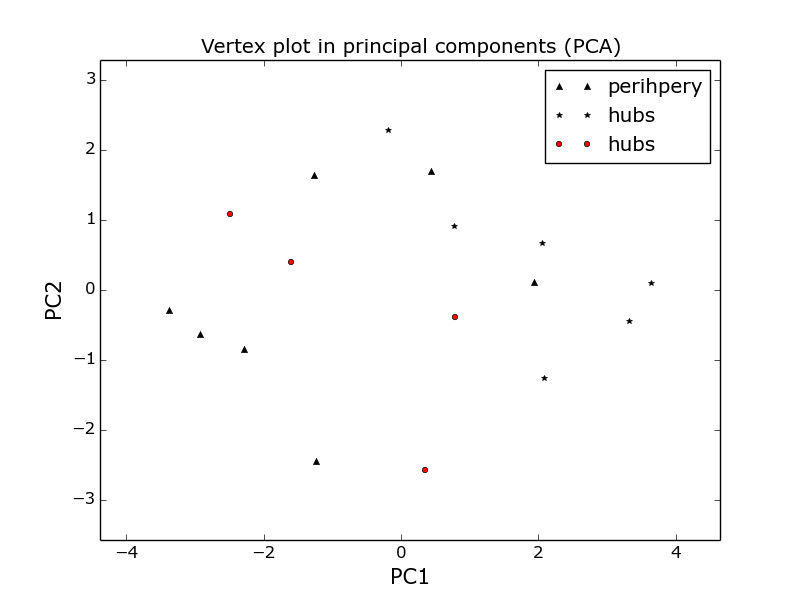
\includegraphics[width=0.3\textwidth]{figs/plot_pca}
% 	\label{fig:formation}
% \end{figure}
Principal components formation of textual and topological metrics
seems to be the less stable of all results reported in this study.
The concentration of dispersion often peaked in the intermediary sector.
% Clustering coefficient was dominant in a principal component almost exclusively
% when the whole network was used for PCA, otherwise it combined more evenly with
% other measures.
% This reveals that clustering coefficient might be a more relevant feature for the complete network
% than for each separate sector.
Components are most often composed of topological or textual features.
Other than that, we observe that PCA is sensitive to metrics included
and should reveal other insights in other settings.
These results are exemplified in Table~\ref{tab:tpca}.

\subsection{Results still to be interpreted}\label{subsec:sii}
%These networks yield diverse characteristics,
%some of which were not of core importance for this step of the research.
%Even so, at least one of these characteristics was found interesting enough to be considered a result and an example of interesting artifacts found.
Histogram differences of incident word sizes with and without repetition of words are constant.
That is, in each email list, when a histogram of word sizes were made with all words written,
and another histogram made with sizes of all \emph{different} words,
the cumulative absolute difference of the two histograms throughout the bins were found constant for all lists analysed.
When all known English words were considered, 
the difference sums up to $\approx 1.0$.
When stopwords are discarded,
the difference found was different, but still constant, slightly above $0.5$.
When only stopwords were considered, the difference is $\approx 0.6$.
When only known English words that does not have Wordnet synsets are used,
this difference is $\approx 1.2$.
We considered this result a number of times in the past years and presented it to other researchers,
but reached no conclusions about its meaning.
Appendix ~\ref{sec:resE} are dedicated to this histogram differences.

\section{Results from visualization}
Results from Versinus are divided in two groups:
observations on features that made it useful for the task of hypothesizing about general properties of human interaction networks,
and the network properties it made possible to grasp.

\subsection{Useful visualization features for dynamic networks}

Among the numerous insights related to Versinus, a few of them seem more fundamental, others seem simply useful.
Such insights were incorporated to Versinus as the result of tests which presented clear benefits within the context of our research.
The following list is an attempt to present them in an importance-first order:
\begin{enumerate}
	\item Vertices need to remain static.
		Even if they move smoothly, one tends to notice solely transient artifacts from the structure.
	\item Very connected sectors (hubs and intermediary) need to be in a curve, otherwise the edges enclose each other and reasoning about the network becomes harsh.
	\item Height and width of a vertex are very informative, specially if measures mapped to them have a strong relation, such as out-degree (mapped to height in Versinus) and in-degree (mapped to width).
	\item The color of nodes is also informative although less than height and weight, as differences in the latter are more noticeable.
	\item An ordering of nodes, related to their fixed position, is very useful. Among all tests, ordering of vertices by degree was considered the most informative, which led to the hub, intermediary and peripheral sectioning of the network delineated in Section~\ref{sectioning}.
		As node position in the layout is fixed throughout an animation which comprises consecutive but distinct network activity, such ordering is done with respect to the resulting network of all the activity.
	Numbering these positions with respect to the order of the vertices in the larger structure (i.e. all $M$ messages) is useful for understanding how much a vertex preserves the position in different scales of activity.
\end{enumerate}

Many other insights were derived from Versinus, such as possible visualization tools, other kind of convenient layouts and glyph elaborations.
These receives dedicated attention in Section~\ref{sec:verref}.

\subsection{Understanding of network properties through Versinus}
A number of hypotheses were drawn about the networks for which Versinus was designed.
As suggested by Palla, Barab\'asi and Vicsek~\cite{barabasiEvo}, stability of participant activity in social networks is more incident in smaller networks.
In accordance with this result, all hubs have intermittent activity in the settings analyzed, except for the email list with the smallest number of participants (the Metareciclagem email list).
The intermitence of hubs was one of the top hypotheses which motivated Versinus development.
The stability of the network structure, concomitant with the instability of the activity of each participant,
motivated a deeper analysis~\cite{stab}.
In doing so, we also found evidence for another hypothesis drawn from Versinus:
that in- and out-degree differences in each vertex are important for network characterization.
Furthermore, the visualization suggests that there are modes of operation of the network.
As an example, the intermediary sector often communicates mostly with the hubs or with the peripheral vertices.
Other hypotheses,
such as discrepancies in the authority and the degree of a vertex,
are numerous but need further research to be valuable.
 
\subsection{Refinement of Versinus}\label{sec:verref}
Versinus was convenient for obtaining insights about how to enhance its layout and use.
It was immediate to think of a tool for using Versinus
in real-time, but less obvious are some ideas about the layout and visual guides. 
To further enable visualization of hubs and intermediary vertex,
the sinusoid can have many periods 
with a decaying frequency.
The upper straight line can also have an oscillating outline.
The two halves of the sinusoidal period could be moved independently.
The waveform need not to be a sinusoid.
One can think of many ways to make more informative glyphs.
Also, visual and auditory signals for specific occurrences can be interesting
(e.g. when a new vertex appears, when one vanishes, when an ordering of vertices changes).
Measures of each vertex can be exposed with a vertical displacement,
to enable multiple measures, to avoid the need to blink the numbers and to keep network visualization free from occlusion.
Working with Versinus has also suggested other kinds of layout for vertices, 
specially geometric figures and iterative force-based methods for positioning vertex in a fixed layout.
The traditional matrix representation of the graphs has been gazed upon as support to Versinus 
as has been some recent approaches to network visualization~\cite{Viz1}.


\section{Linked data results}
\label{outline}
Current results include data selection and preparation for knowledge discovery.
In this respect, the main result is the data made available, which enables benchmarking of scientific results
and easy experimentations.
Secondary results include data outline through figures and tables,
software support and example SparQL queries.

\subsection{Standardization}
The data is embedded into standard URIs and triples, i.e. translated to RDF.
URIs are built in the namespace \url{http://purl.org/socialparticipation/participationontology/}
which are identified herein with the prefix \textttt{po:}.
Classes and properties are built by adding a suffix to the root,
as in the class \textttt{po:Participant} or in the property \textttt{po:text}.
Classes have ``UpperCamelCase'' suffixes while properties have ``lowerCamelCase'' suffixes.
All class instances, such as participants, messages, friendships and
interactions, are linked to
snapshots through the triple \textttt{<instance> po:snapshot <snapshot\_uri>}.
Message texts, including comments, are objects in the triple: \textttt{<message\_id> po:text <message\_text>}.
Preprocessed texts are objects of triples: \textttt{<message\_id> po:cleanText <message\_text>}.
More specialized predicates are used for delivering text when necessary,
such as \textttt{po:htmlBodyText} and \textttt{po:cleanBodyText} used
for ParticipaBR articles (instances of the class \textttt{po:Article}.
A participant URI is unique throughout the provenance (e.g. the same for
the same participant in all Twitter snapshots).
To enable annotations which differ when the snapshot changes,
\textttt{po:Observation} class instances are used in the triple
\textttt{<participant\_uri> po:observation <observation\_uri>}.
The observation instances are then linked to the snapshot and the
data.

Instances are built on top of the class they derive from plus a hashtag character,
a provenance string (e.g. \textttt{facebook-legacy} or
\textttt{participabr-legacy}) of the snapshot they refer to, and an identifier;
i.e. \textttt{po:Participant\#<provenance-legacy>-<id>}.
All snapshot URIs follow the formation rule: \textttt{po:<SnapshotProvenance>\#<snapshot\_id>}.
All snapshot ids follow the formation rule: \textttt{<platform>-legacy-<further\_identifier>}; e.g.
\textttt{irc-legacy-labmacambira} or
\textttt{email-legacy-linux.audio.devel1-20000}.

\subsection{Data outline}
The database consists of 34,120,026 triples, 3,172,927 edges yield by interactions or relations, 382,568 participants and 253,155,020 characters. Among all snapshots, 63 are ego snapshots, 54 are group snapshots; 49 have interaction edges, 89 have friendship edges; 43 have text content from messages.



\begin{table*}[h!]
\begin{center}
\caption{Number of snapshots from each provenance.}
\begin{tabular}{| l | c |}\hline
\textbf{social protocol} & \textbf{number of snapshots} \\\hline\hline
Algorithmic Autoregulation & 3 \\\hline
Cidade Democrática & 1 \\\hline
Email & 4 \\\hline
Facebook & 88 \\\hline
IRC & 4 \\\hline
ParticipaBR & 1 \\\hline
Twitter & 16 \\\hline\hline
all & 117 \\\hline
\end{tabular}\end{center}
\end{table*}
% stats:
%% number of triples
%% number of edges
%% number of chars
%% number of users
% diagrams in the supporting information file
\subsection{Software tools}
The database is released with software for rendering itself, analyses and
multimedia artifacts.
\subsubsection{Triplification routines}
For each social platform there is a \emph{triplification} routine,
i.e. a script for translating data to RDF.
Original formats and further observations are presented in
Table~\ref{tab:provenance}.
\begin{table*}[h!]\scriptsize
	\begin{center}
		\caption{Social platforms, original formats and further observations for
		the database.}\label{tab:provenance}
		\begin{tabular}{| l || p{3cm} | p{3cm} | c |}\hline
			\textbf{social platform} & \textbf{original format} & \textbf{further observations} & \textbf{toolbox} \\\hline\hline
				AA & MySQL and MongoDB databases; IRC text logs & donated by AA users & Participation~\cite{participation} \\\hline
				    Cidade Democrática & MySQL database & donated by admins & Participation \\\hline
					Email & mbox & obtained through Gmane public database & Gmane~\cite{gmane} \\\hline
					    Facebook & GDF, GML and TAB & obtained through Netvizz~\cite{netvizz} & Social~\cite{social} \\\hline
						IRC & plain text log & obtained through Supybot logging & Social \\\hline
						    ParticipaBR & PostgreSQL database & donated by admins & Participation \\\hline
							Twitter & JSON & obtained through Twitter streaming API & Social \\\hline
		\end{tabular}
\begin{flushleft}
		Source: Prepared by the authors.\
\end{flushleft}
	\end{center}
	\end{table*}                    
\subsubsection{Topological and textual analysis}\label{ana}
Routines are available for taking the topological and textual measures from
the database.
Auxiliary routines, such as performing principal component analysis
and taking Kolmogorov-Smirnov measures, are available
to ease pattern recognition.
All the analysis routines used for this thesis are in these publicly accessible scripts.

\subsubsection{Multimedia rendering}\label{media}
It is a core purpose of the framework to provide routines for rendering
audiovisualizations of the data.
Social structures are rendered into music, images and video animations
through the Percolation toolbox~\cite{percolation} in association with
the Music and Visuals toolboxes~\cite{music,visuals}.

\subsubsection{Migration from deprecated toolboxes}
Routines mentioned in Sections~\ref{ana} and~\ref{media} are being migrated from deprecated
toolboxes~\cite{gmaneLegacy,percolationLegacy} into newly designed
toolboxes~\cite{percolation,visuals}.

\subsection{Diagrams of the data and auxiliary tables}
The database exploration can be assisted through diagrams which expose
the structure from each provenance.
Such diagrams are exemplified in the Appendix~\ref{losd} and 
fully available in a dedicated article~\cite{losd}
with some tables to make it easier to understand the data provided.
A simplified example is given in Figure~\ref{dia} where the friendship
structure of the Facebook snapshots are exposed.

	\begin{figure}[!ht]
		\centering
			    \caption{A diagram of the structure involved in the friendship networks
				of the Facebook snapshots.
				A green edge denotes an OWL existential class restriction;
				an inverted nip denotes an OWL universal class restriction;
				a full (non-dashed) edge denotes an OWL functional property axiom.
				Further information and complete diagrams for each provenance are in the dedicated article~\cite{losd}.}\label{dia}
			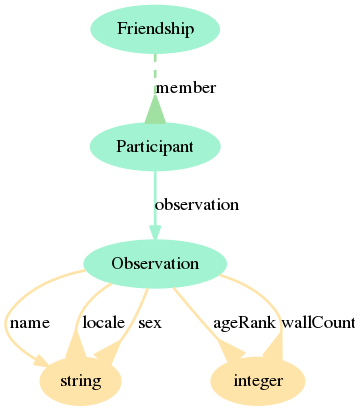
\includegraphics[width=0.5\textwidth]{ontologies/facebook-legacy-AntonioAnzoategui18022013Friendship.ttl/draw}
\begin{flushleft}
		Source: Prepared by the authors.\
\end{flushleft}
	\end{figure}


	\subsection{SPARQL queries}\label{queries}
	There are numerous useful and general purpose SPARQL queries to be performed against the database.
	Here we write some of such queries selected by their simplicity and potential to be varied.
	All queries assume the use the preamble \textttt{PREFIX po: <http://purl.org/socialparticipation/po/>}.
	\begin{enumerate}[leftmargin=0cm]
		\item Retrieve the number of participants:\\
			\textttt{SELECT (COUNT(DISTINCT ?author) as ?c) WHERE \{
				?author a po:Participant . \} }
			\item Retrieve the number of relations, be them interactions or
				friendships:\\
														\textttt{SELECT (COUNT(?interaction) as ?c) WHERE \{\\
																    \h \{ ?interaction a po:Friendship \} UNION \{ ?interaction
																			a po:Interaction \} UNION\\
																					    \h \{ ?interaction po:retweetOf
																								?message \} UNION \{ ?interaction po:replyTo ?message
																										    \}\\
																													\h UNION \{ ?interaction po:directedTo ?participant
																															    \}\\ \} }
																														    \item Retrieve all text produced by an specific user:\\
																															    \textttt{SELECT (CONCAT(?text) as ?texts) WHERE \{\\
																																					\h ?activity po:author <user\_uri> . ?activity po:text ?text .\\
																																					    \}}
																																				    \item List 1000 users (URIs and names) with the most friendships and the number of
																																					    friendships in descending order by the number of friendships:\\
																																										    \textttt{SELECT DISTINCT ?participant (COUNT(?friendship)
																																												as ?c) WHERE \{\\
																																														\h ?friendship a po:Friendship . ?friendship po:member ?participant . \\
																																															    \} ORDER BY DESC(?c) LIMIT 1000}
																																														    \item Retrieve text messages with the word ``pineapple'' (case insensitive):\\
																																															    \textttt{SELECT ?text WHERE \{ \\
																																																					    \h ?activity po:text ?text . FILTER regex(?text, 'pineapple', 'i')\\
																																																						\}}
																																																					\item List participants and respective full names whose name has the substring ``Amanda'':\\
																																																						\textttt{SELECT DISTINCT ?participant ?name WHERE \{\\
																																																							\h ?participant po:observation ?obs . ?obs po:name ?name .\\
																																																							    \h FILTER regex(?name, 'Amanda', 'i') \\
																																																								\}}
																																																							\item Return all pairs of friends of a participant which are friends themselves:\\
																																																								\textttt{SELECT DISTINCT ?friend1 ?friend2 WHERE \{\\
																																																									 \h       ?friendship1 po:member <participant\_uri> .  ?friendship1 po:member ?friend1 .\\
																																																									      \h       ?friendship2 po:member <participant\_uri> .  ?friendship2 po:member ?friend2 .\\
																																																										   \h       ?friendship3 po:member ?friend1 .  ?friendship3 po:member ?friend2 .\\
																																																										       \}}
																																																									       \item Return all interactions from replies in a snapshot:\\
																																																										       \textttt{SELECT ?from ?to WHERE \{\\
																																																												     \h  ?message1 po:snapshot <snapshot\_uri> .  ?message2 po:replyTo ?message1 .\\
																																																													       \h  ?message1 po:author ?from .  ?message2 po:author ?to .\\
																																																														   \}}
	\end{enumerate}

	\subsection{License issues}
	% Facebook, Twitter, IRC, Gmane, Participa, CD, AA.
	The database presented in this thesis is released under public domain.
	Computer scripts are in git repositories and PyPI Python packages, also under public domain.
	Although most data is already in open licenses (Twitter, Email, Participabr, Cidade Democrática, and AA data), IRC and Facebook data was collected
	and donated by the individuals which yield the data.
	This rises the understanding of the right to study such data as the right to access the self,
	in parity with anthropological endeavors~\cite{antphy,antphy2}.


\subsection{Data-driven ontology synthesis}
OWL Ontologies are critical tools to describe taxonomies and the
structure of knowledge.
Most ontologies are created by domain experts even though there often is data they
organize that is given by a software system and which has a predefined
structure.  

We developed a simple ontology synthesis method that probes
the ontological structure in data with
SPARQL queries and post-processing.
The results are OWL code and diagrams which are 
exemplified in the Appendix~\ref{losd} and 
fully available in a dedicated article~\cite{losd}.
The method can be extended to comprise further OWL axioms and restrictions,
but is currently performed to fit present needs with maximum simplicity.
Present needs are limited to informative figures and
the steps implemented are as follows:
\begin{enumerate}[leftmargin=0cm]
	\item Obtain all distinct classes with the query:\\
		\textttt{SELECT DISTINCT ?class\_uri WHERE \{ ?s a ?class\_uri \}}
	\item For each class, obtain the properties that occur as predicates in triples where the subject is an instance of the class:\\
		\textttt{SELECT DISTINCT ?property\_uri WHERE \{ ?s a <class\_uri> . ?s ?property\_uri ?o . \}}\\
					Such properties are used to assert existential and universal restrictions for the class.
				\item Compare the total number of individuals (\textttt{?cs1}) of the class (\textttt{class\_uri}) with
					the number of such individuals (\textttt{?cs2}) that are subjects of at least one triple where 
							the predicate is the property (\textttt{property\_uri}).
								If the numbers match, there is an existential restriction for the class. The queries are:\\
									\textttt{SELECT (COUNT(DISTINCT ?s) as ?cs1) WHERE \{ ?s a <class\_uri> \}}\\
										\textttt{SELECT (COUNT(DISTINCT ?s) as ?cs) WHERE \{\\
											\h ?s a <class\_uri>. ?s <property\_uri> ?o .\\ \}}
										\item Find the number of instances which are subjects of triples where the predicate is the property but are not instances of the class.
											If there is zero of such instances, there is an universal restriction:\\
													\textttt{SELECT (COUNT(DISTINCT ?s)=0 as ?cs) WHERE \{\\
														\h ?s <property\_uri> ?o . ?s a ?ca . FILTER(str(?ca) != 'class\_uri')\\ \}}
													\item To keep a record of the restrictions (and occurring triples), get all object classes or datatypes where the subject is an instance of the class and the predicate is the property:\\
														\textttt{SELECT DISTINCT ?co (datatype(?o) as ?do) WHERE \{\\
																	\h ?s a <class\_uri>. ?s <property\_uri> ?o . OPTIONAL \{ ?o a ?co . \}\\
																	\}}
																\item Obtain all distinct properties:\\
																	\textttt{SELECT DISTINCT ?p WHERE \{ ?s ?p ?o \}}
																\item Check if each property is functional, i.e. if it
																	occurs at most once with each subject.
																							This is performed by counting the objects and further verifying
																								that they are at most one. The query is:\\
																									\textttt{SELECT DISTINCT (COUNT(?o) as ?co) WHERE \{ ?s
																										    <property\_uri> ?o \} GROUP BY ?s}
																									    \item For each property, find the incident range and domain with the
																										    queries:\\
																														\textttt{SELECT DISTINCT ?co (datatype(?o) as ?do) WHERE \{\\
																																	\h ?s <property\_uri> ?o . OPTIONAL \{ ?o a ?co . \}\\\}} \\
																																		and \\
																																			\textttt{SELECT DISTINCT ?cs WHERE \{ ?s <property\_uri> ?o . ?s a ?cs . \}}
																																		\item Render diagrams as exposed in the next section and in the Supporting Information file.
\end{enumerate}


